\documentclass[11pt,letterpaper]{article}

\usepackage{fancyhdr}
\usepackage{lastpage}
\usepackage[T1]{fontenc}
\usepackage[latin1]{inputenc}
\usepackage[cyr]{aeguill}
\usepackage[colorlinks=true]{hyperref}
\usepackage{textpos}
\usepackage{graphicx}
\usepackage[english]{babel}
\usepackage{color}
\usepackage{array}
\usepackage{enumitem}
\usepackage{amsmath}
\usepackage{amssymb}
\usepackage{amsthm}
\usepackage{multicol}   % For side-by-side formatting

\usepackage{framed}
%\usepackage{enumerate}
\definecolor{shadecolor}{gray}{0.9}

\usepackage{xcolor}

\definecolor{problemcolor}{rgb}{0.2, 0.1, 0.8} % Define color for Problem
\definecolor{solproblemcolor}{rgb}{0.8, 0.2, 0.2} % Define color for Solution to Problem

\theoremstyle{definition}
\newtheorem{prob}{\textcolor{problemcolor}{Problem}}  % Color for Problem
\newtheorem{solprob}{\textcolor{solproblemcolor}{Solution to Problem}}  % Col

\usepackage{geometry}
\geometry{left=7mm,top=12mm,body={190mm,279.4mm}}
\usepackage{amsmath}
\usepackage{amssymb}
\usepackage{amsfonts}
\usepackage{dsfont}
\usepackage{amsthm}
\usepackage{float}


%\usepackage{enumerate}
\usepackage{fancyhdr}
\pagestyle{fancy}


\renewcommand{\headrulewidth}{0pt}
\renewcommand{\footrulewidth}{4pt}
\allowdisplaybreaks


\newcommand{\session}{Fall 2025}




\def\0{{\mathbf 0}}
\def\1{{\mathbf 1}}

\def\a{{\mathbf a}}
\def\b{{\mathbf b}}
\def\c{{\mathbf c}}
\def\d{{\mathbf d}}
\def\e{{\mathbf e}}
\def\f{{\mathbf f}}
\def\g{{\mathbf g}}
\def\h{{\mathbf h}}
\def\i{{\mathbf i}}
\def\j{{\mathbf j}}
\def\k{{\mathbf k}}
\def\l{{\mathbf l}}
\def\m{{\mathbf m}}
\def\n{{\mathbf n}}
\def\o{{\mathbf o}}
\def\p{{\mathbf p}}
\def\q{{\mathbf q}}
\def\r{{\mathbf r}}
\def\s{{\mathbf s}}
\def\t{{\mathbf t}}
\def\u{{\mathbf u}}
\def\v{{\mathbf v}}
\def\w{{\mathbf w}}
\def\x{{\mathbf x}}
\def\y{{\mathbf y}}
\def\z{{\mathbf z}}

\def\A{{\mathbf A}}
\def\B{{\mathbf B}}
\def\C{{\mathbf C}}
\def\D{{\mathbf D}}
\def\E{{\mathbf E}}
\def\F{{\mathbf F}}
\def\G{{\mathbf G}}
\def\F{{\mathbf F}}
\def\H{{\mathbf H}}
\def\I{{\mathbf I}}
\def\J{{\mathbf J}}
\def\K{{\mathbf K}}
\def\L{{\mathbf L}}
\def\M{{\mathbf M}}
\def\N{{\mathbf N}}
\def\O{{\mathbf O}}
\def\P{{\mathbf P}}
\def\Q{{\mathbf Q}}
\def\R{{\mathbf R}}
\def\S{{\mathbf S}}
\def\T{{\mathbf T}}
\def\U{{\mathbf U}}
\def\V{{\mathbf V}}
\def\W{{\mathbf W}}
\def\X{{\mathbf X}}
\def\Y{{\mathbf Y}}
\def\Z{{\mathbf Z}}


\def\rE{{\text{E}}}
\def\rPr{{\text{Pr}}}
\def\Tr{{\text{Tr}}}
\def\vec{{\textrm{vec}}}
\def\ie{{\textit{i.e.}}}
\def\eg{{\textit{e.g.}}}


\def\cA{{\mathcal A}}
\def\cB{{\mathcal B}}
\def\cC{{\mathcal C}}
\def\cD{{\mathcal D}}
\def\cE{{\mathcal E}}
\def\cF{{\mathcal F}}
\def\cG{{\mathcal G}}
\def\cH{{\mathcal H}}
\def\cI{{\mathcal I}}
\def\cK{{\mathcal K}}
\def\cL{{\mathcal L}}
\def\cM{{\mathcal M}}
\def\cN{{\mathcal N}}
\def\cO{{\mathcal O}}
\def\cP{{\mathcal P}}
\def\cQ{{\mathcal Q}}
\def\cR{{\mathcal R}}
\def\cS{{\mathcal S}}
\def\cT{{\mathcal T}}
\def\cU{{\mathcal U}}
\def\cV{{\mathcal V}}
\def\cW{{\mathcal W}}
\def\cX{{\mathcal X}}
\def\cY{{\mathcal Y}}
\def\cZ{{\mathcal Z}}


\def\bphi{{\pmb{\phi}}}
\def\bpsi{{\pmb{\psi}}}
\def\bphi{{\pmb{\phi}}}
\def\bpsi{{\pmb{\psi}}}
\def\balpha{{\boldsymbol \alpha}}
\def\bbeta{{\boldsymbol \beta}}
\def\bvarphi{{\boldsymbol \varphi}}
\def\bPhi{{\boldsymbol \Phi}}


\def\bcdot{{\;\boldsymbol{\cdot}\;}}


\oddsidemargin 0pt
\topmargin 0pt
\textwidth 6.5in
\textheight 8.1in
\newtheorem{exemple}{Exemple}

\definecolor{bleu_poly}{RGB}{65,170,230}
\definecolor{vert_poly}{RGB}{140,200,60}
\definecolor{orange_poly}{RGB}{250,150,30}
\definecolor{rouge_poly}{RGB}{185,30,50}
\definecolor{gris_poly}{RGB}{166,168,171}

\newcommand{\matlab}{\textsc{Matlab} }
\newcommand{\simulink}{\textsc{Simulink} }

\title{\vspace{-5.5cm} \noindent\makebox[\linewidth]{\color{rouge_poly}{\rule{\textwidth}{1.5pt}}}
	\begin{center}
		\begin{tabular}{m{8cm}m{7cm}}
			\textbf{ \huge Homework 1}  & 
\includegraphics[width=0.4\textwidth]{York_logo}
		\end{tabular}
	\end{center}
	\noindent\makebox[\linewidth]{\color{rouge_poly}{\rule{\textwidth}{1.5pt}}}
	\\ \ \\
	\LARGE EECS 2200 - Electrical Circuits}\vspace{0.01mm}


\author{\session\vspace{3mm} \\ Departement of Electrical Engineering and Computer Science \\\vspace{8mm}
	York University\\
	\textbf{Instructor:} Houshang Karimi}

\date{\textbf{Due Date:} September 22, 2025\\[5mm]
	\textbf{Last Update:} \today}





\pagestyle{fancy}

\usepackage{lastpage}
%\rfoot{Page \thepage~of \pageref{LastPage}}

\lfoot{\session}
\cfoot{~~~~~~~EECS 2200 - Electrical Circuits ~~~~~~~ Page \thepage~of \pageref{LastPage}}




\chead{}
\lhead{\emph{Homework 1}}
\rhead{\includegraphics[width=3.5cm]{York_Logo}}
%\rhead{\vspace{-1cm}\includegraphics[width=2cm]{polytechnique_genie_droite_fr_cmyk}}
\renewcommand{\headrulewidth}{0.4pt}
\renewcommand{\footrulewidth}{0.4pt} 
\setlength{\headheight}{45pt}

\graphicspath{{Fig/}}

\newcounter{numq}
\setcounter{numq}{1}    % Value is 0

%\setenumerate[1]{label=(\alph*), leftmargin=3em}

\begin{document}
	\maketitle
	\vspace{-5mm}

%\noindent\makebox[\linewidth]{\color{rouge_poly}{\rule{\textwidth}{1.3pt}}}
%%%%	******************%
%\noindent\textbf{Note:} Writing your homework in \textbf{LaTeX} will be rewarded with bonus points! 

%\begin{enumerate}[label=(\roman*)]
%	\item Writing your homework in \textbf{LaTeX} will be rewarded with bonus points! 
%	\item Submit your MATLAB simulation files (.m files) along with your homework solutions. 
%\end{enumerate} 
\noindent\makebox[\linewidth]{\color{rouge_poly}{\rule{\textwidth}{1.3pt}}}	
%%%%	******************%
	
	\vspace{5mm}
	
	\centering
	\fbox{\begin{minipage}{30em}
			\vspace{4mm}
			First Name: Thomas\\\vspace{2mm}
			
			Last Name: Newman\\\vspace{2mm}
			
			Student Number: $221224662$
			\vspace{3mm}
	\end{minipage}}
	
	\vspace{-0.1mm}
	
	%\centering
	\begin{table}[!h]
	%	\large
		\centering
		\renewcommand{\arraystretch}{2}
		\hspace{-0.02cm}\begin{tabular}{|l|l|l|l|l|l|l|l|l|l|l|l|l|l|l|l|l|l|l|}
			\cline{1-17}
			Problem		& $P_1$ & $P_2$ & $P_3$ & $P_4$  & $P_5$  & $P_6$ &  $P_7$  & $P_8$ &  $P_9$  & $P_{10}$  & $P_{11}$  &  $P_{12}$  &  $P_{13}$  &  $P_{14}$  &  $P_{15}$  &   Total  \\ \cline{1-17}
			Mark	    	&  $\dfrac{}{~5~}$ &  $\dfrac{}{~5~}$ &  $\dfrac{}{~5~}$ &  $\dfrac{}{~5~}$ & $\dfrac{}{~5~}$ & $\dfrac{}{~5~}$  & $\dfrac{}{~5~}$   & $\dfrac{}{~5~}$   & $\dfrac{}{~5~}$   & $\dfrac{}{~5~}$   & $\dfrac{}{~5~}$   & $\dfrac{}{~5~}$   &$\dfrac{}{~5~}$   &$\dfrac{}{~5~}$   &$\dfrac{}{~5~}$   &  $\dfrac{}{~75~}$ \\ \cline{1-17}
			%		&  &  &   \\ \cline{1-4}
		\end{tabular}
		\renewcommand{\arraystretch}{1}
	\end{table}

	\noindent\makebox[\linewidth]{\color{rouge_poly}{\rule{\textwidth}{1.5pt}}}
	
\begin{enumerate}
	\item[{\textbf{CLO1:}}] \textbf{Analyze resistive circuits using basic laws (node and loop analysis, Thevenin, Norton's, superposition).}
	\item[{\textbf{CLO2:}}] \textbf{Determine the transient response of RC, RL, and RLC circuits.}
	\item[{\textbf{CLO3:}}] \textbf{Analyze AC circuits in steady state using the phasor method.}
	\item[{\textbf{CLO4:}}] \textbf{Use basic tools such as MATLAB and SPICE for circuit analysis.}
	\item[{\textbf{CLO5:}}] \textbf{Measure basic electrical signals using electronic measurement equipment in a lab setting.}
\end{enumerate}

	\noindent\makebox[\linewidth]{\color{rouge_poly}{\rule{\textwidth}{1.5pt}}}
	\newpage
%%%%%%%%%%%%%%%%%%%%%%%%%%%%%%%%%%%%%%%%%%%%%%%%%%%%%%%%%%%%%%%%%%%%%%%%%%%%%%%%%%%%%%%%%%%%%%%%%%%%%%%%%%%%%%%%%%%%%%%%%%%%%%%%%%%%%%%%%%%%%%
%%%%%%%%%%%%%%%%%%%%%%%%%%%%%%%%%%%%%%%%%%%%%%%%%%%%%%%%%%%%%%%%%%%%%%%%%%%%%%%%%%%%%%%%%%%%%%%%%%%%%%%%%%%%%%%%%%%%%%%%%%%%%%%%%%%%%%%%%%%%%%
%%%%%%%%%%%%%%%%%%%%%%%%%%%%%%%%%%%%%%%%%%%%%%%%%%%%%%%%%%%%%%%%%%%%%%%%%%%%%%%%%%%%%%%%%%%%%%%%%%%%%%%%%%%%%
%%%%%%%%%%%%%%%%%%%%%%%%%%%%%%%%%%%%%%%%%%%%%%%%%%%%%%%%%%%%%%%%%%%%%%%%%%%%%%%%%%%%%%%%%%%%%%%%%%%%%%%%%%%%%
%%%%%%%%%%%%%%%%%%%%%%%%%%%%%%%%%%%%%%%%%%%%%%%%%%%%%%%%%%%%%%%%%%%%%%%%%%%%%%%%%%%%%%%%%%%%%%%%%%%%%%%%%%%%%
%%%%%%%%%%%%%%%%%%%%%%%%%%%%%%%%%%%%%%%%%%%%%%%%%%%%%%%%%%%%%%%%%%%%%%%%%%%%%%%%%%%%%%%%%%%%%%%%%%%%%%%%%%%%%
	

\begin{prob}\label{pb:p1} The current in a circuit element is  
\[
	i(t) =
	\begin{cases}
		0 & t < 2 \\[6pt]
		2 & 2 < t < 4 \\[6pt]
		-1 & 4 < t < 8 \\[6pt]
		0 & t > 8
	\end{cases}
\]
where the units of current are amperes (A) and the units of time are seconds (s).  
	Determine the total charge that has entered the circuit element for $t \geq 0$.
\end{prob}

\noindent\makebox[\linewidth]{\color{rouge_poly}{\rule{\textwidth}{1.3pt}}}

\begin{solprob} \text{}\\

    \[
q(t) = \int_{0}^{t} i(t)\,dt
\]

Thus, the total charge that has entered for \(t \geq 0\) is

\[
Q_{\text{net}} = \int_{0}^{\infty} i(t)\,dt
= \int_{2}^{4} 2 \, dt + \int_{4}^{8} (-1) \, dt
= 2(4-2) - 1(8-4)
= 4 - 4
= 0 \ \text{C}.
\]

So the element received \(4 \ \text{C}\) and then \(4 \ \text{C}\) left, giving a net charge of
\[
Q_{\text{net}} = 0 \ \text{C}.
\]

    
\end{solprob}

\noindent\makebox[\linewidth]{\color{rouge_poly}{\rule{\textwidth}{1.3pt}}}	
%%%%%%%%%%%%%%%%%%%%%%%%%%%%%%%%%%%%%%%%%%%%%%%%%%%%%%%%%%%%%%%%%%%%%%%%%%%%%%%%%%%%%%%%%%%%%%%%%%%%%%%%%%%%%%
%%%%%%%%%%%%%%%%%%%%%%%%%%%%%%%%%%%%%%%%%%%%%%%%%%%%%%%%%%%%%%%%%%%%%%%%%%%%%%%%%%%%%%%%%%%%%%%%%%%%%%%%%%%%%%
%%%%%%%%%%%%%%%%%%%%%%%%%%%%%%%%%%%%%%%%%%%%%%%%%%%%%%%%%%%%%%%%%%%%%%%%%%%%%%%%%%%%%%%%%%%%%%%%%%%%%%%%%%%%%%
%%%%%%%%%%%%%%%%%%%%%%%%%%%%%%%%%%%%%%%%%%%%%%%%%%%%%%%%%%%%%%%%%%%%%%%%%%%%%%%%%%%%%%%%%%%%%%%%%%%%%%%%%%%%%%

\begin{prob}\label{pb:p2} 
	Figure~\ref{fig_pw_vi} shows the current through and the voltage  
	across an element. 
	\begin{enumerate}[label=(\alph*)]
		\item Sketch the power delivered to the element for $t > 0$.
		\item Find the total energy absorbed by the element for the period $0 < t < 4\,\text{s}$.
	\end{enumerate}
\end{prob}

\begin{figure}[H]
	\centering
	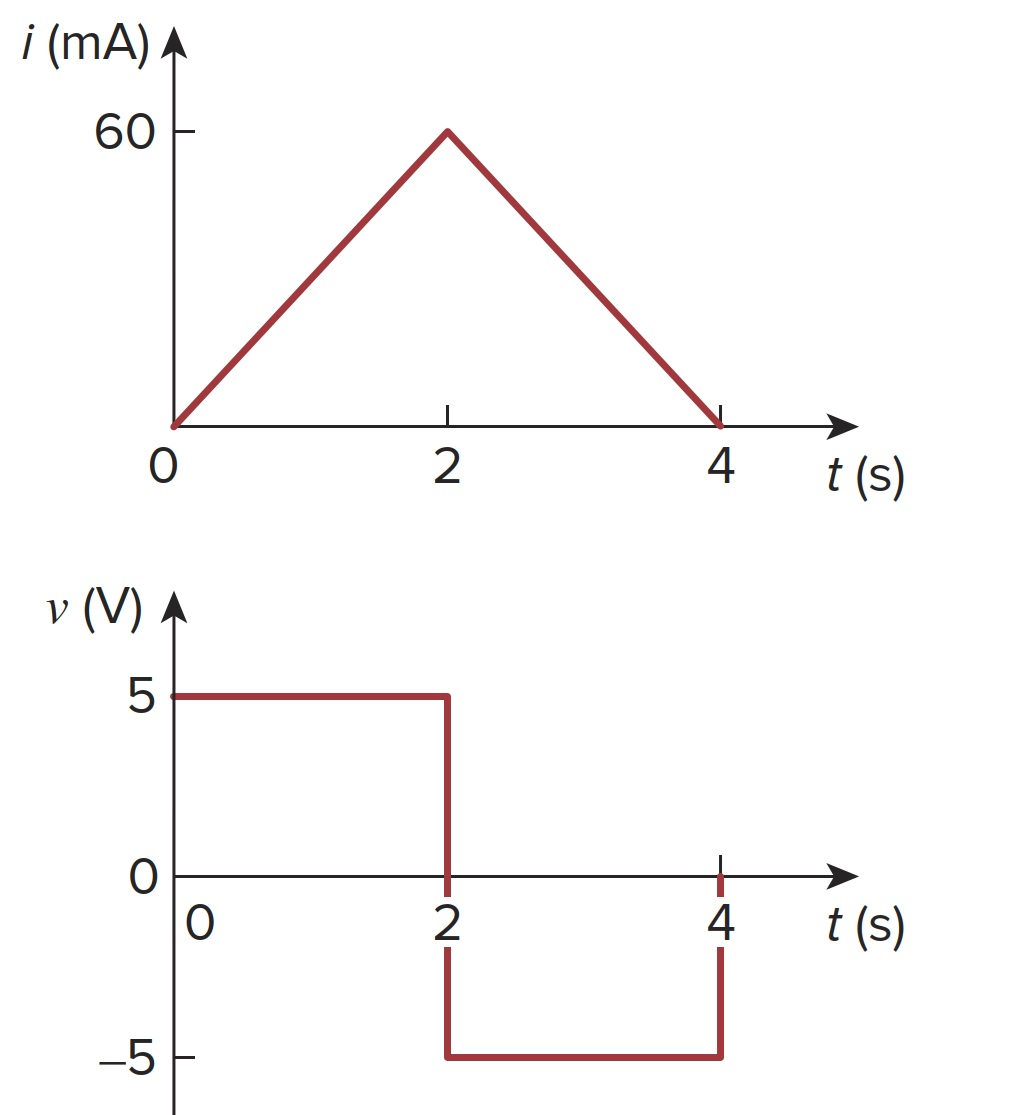
\includegraphics[width=0.4\textwidth]{fig_pw_vi.jpg}
	\caption{Current through and voltage across an element.}
	\label{fig_pw_vi}
\end{figure}


\noindent\makebox[\linewidth]{\color{rouge_poly}{\rule{\textwidth}{1.3pt}}}

\begin{solprob} \text{}\\
    \[
    w = \int_{0}^{\infty} vi \, dt \, + w(0)
    \]

    \begin{enumerate}[label=(\alph*)]
		\item  Sketch the power delivered to the element for $t > 0$.
        \begin{figure}[H]
            \centering
            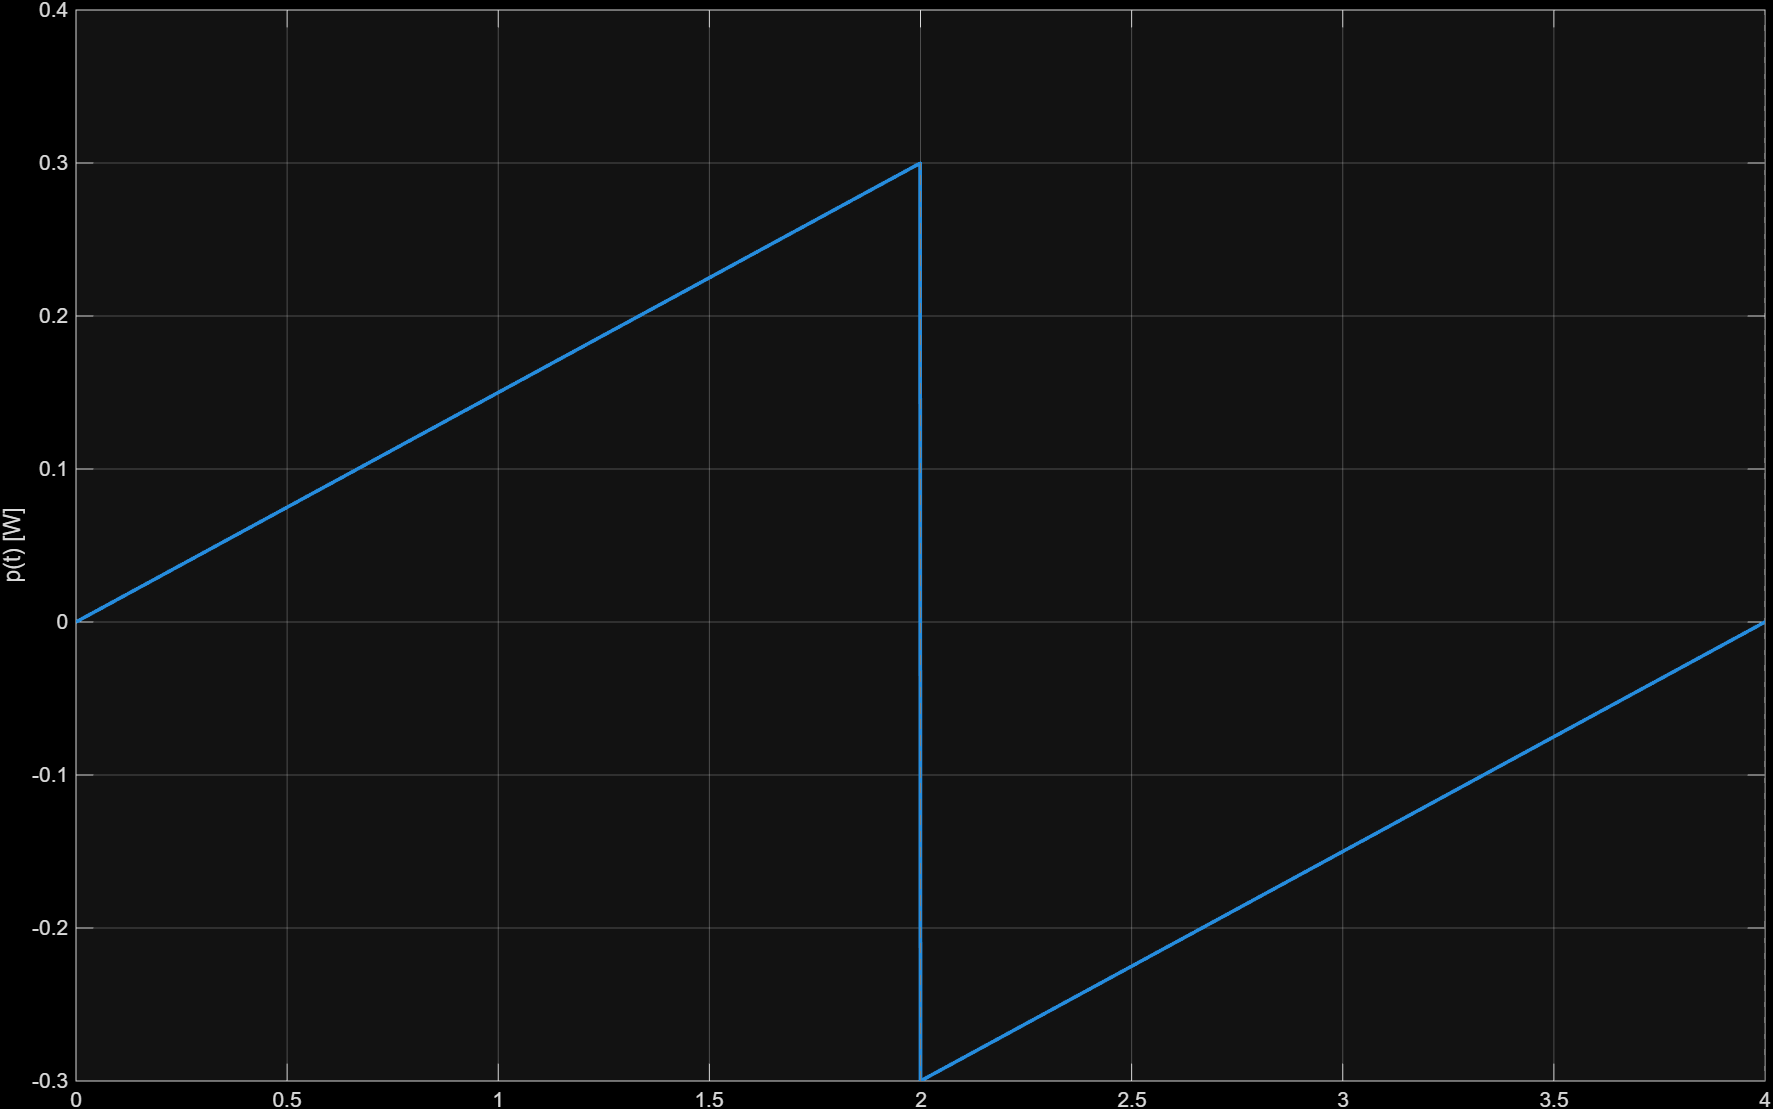
\includegraphics[width=0.75\textwidth]{EECS2200 - Homework1- 1a.png}
            \caption{A Matlab Sketch of the power delivered to the element}
        \end{figure}
		\item Find the total energy absorbed by the element for the period $0 < t < 4\,\text{s}$.
        \[v(t) = \begin{cases}
        +5\, \{0 < x < 2\} \\
        -5\,\{2<x<4\}
        \end{cases}\]
        \[i(t) = \begin{cases}
        0.03t\, \{0 < x < 2\} \\
        0.12-0.03t\,\{2<x<4\}
        \end{cases}\]
        \[p(t) = \begin{cases}
        (+5)(0.03t) = 0.15t\, \{0 < x < 2\} \\
        (-5)(0.12 - 0.03t) = 0.60-0.15t\,\{2<x<4\}
        \end{cases}\]
        \[w_\text{net} = \int_{0}^{4} p(t) \, dt =\int_{0}^{2} 0.15t \, dt + \int_{2}^{4} 0.60-0.15t\,dt\]
        \[w_\text{net} = ((0.15)(2)-(0.15)(0)) + ((0.60-0.15(4))-(0.60-0.15(2)))= 0.30 J - 0.30 J = 0J\]
	\end{enumerate}
\end{solprob}

\noindent\makebox[\linewidth]{\color{rouge_poly}{\rule{\textwidth}{1.3pt}}}	
%%%%%%%%%%%%%%%%%%%%%%%%%%%%%%%%%%%%%%%%%%%%%%%%%%%%%%%%%%%%%%%%%%%%%%%%%%%%%%%%%%%%%%%%%%%%%%%%%%%%%%%%%%%%%%
%%%%%%%%%%%%%%%%%%%%%%%%%%%%%%%%%%%%%%%%%%%%%%%%%%%%%%%%%%%%%%%%%%%%%%%%%%%%%%%%%%%%%%%%%%%%%%%%%%%%%%%%%%%%%%
%%%%%%%%%%%%%%%%%%%%%%%%%%%%%%%%%%%%%%%%%%%%%%%%%%%%%%%%%%%%%%%%%%%%%%%%%%%%%%%%%%%%%%%%%%%%%%%%%%%%%%%%%%%%%%
%%%%%%%%%%%%%%%%%%%%%%%%%%%%%%%%%%%%%%%%%%%%%%%%%%%%%%%%%%%%%%%%%%%%%%%%%%%%%%%%%%%%%%%%%%%%%%%%%%%%%%%%%%%%%%

\begin{prob}\label{pb:p3}
	Find $V_o$, $I_o$, $V_1$, $V_2$, $I_3$ and the power absorbed by each element in the circuit of Fig.~\ref{fig_1_31}.
\end{prob}

\begin{figure}[H]
	\centering
	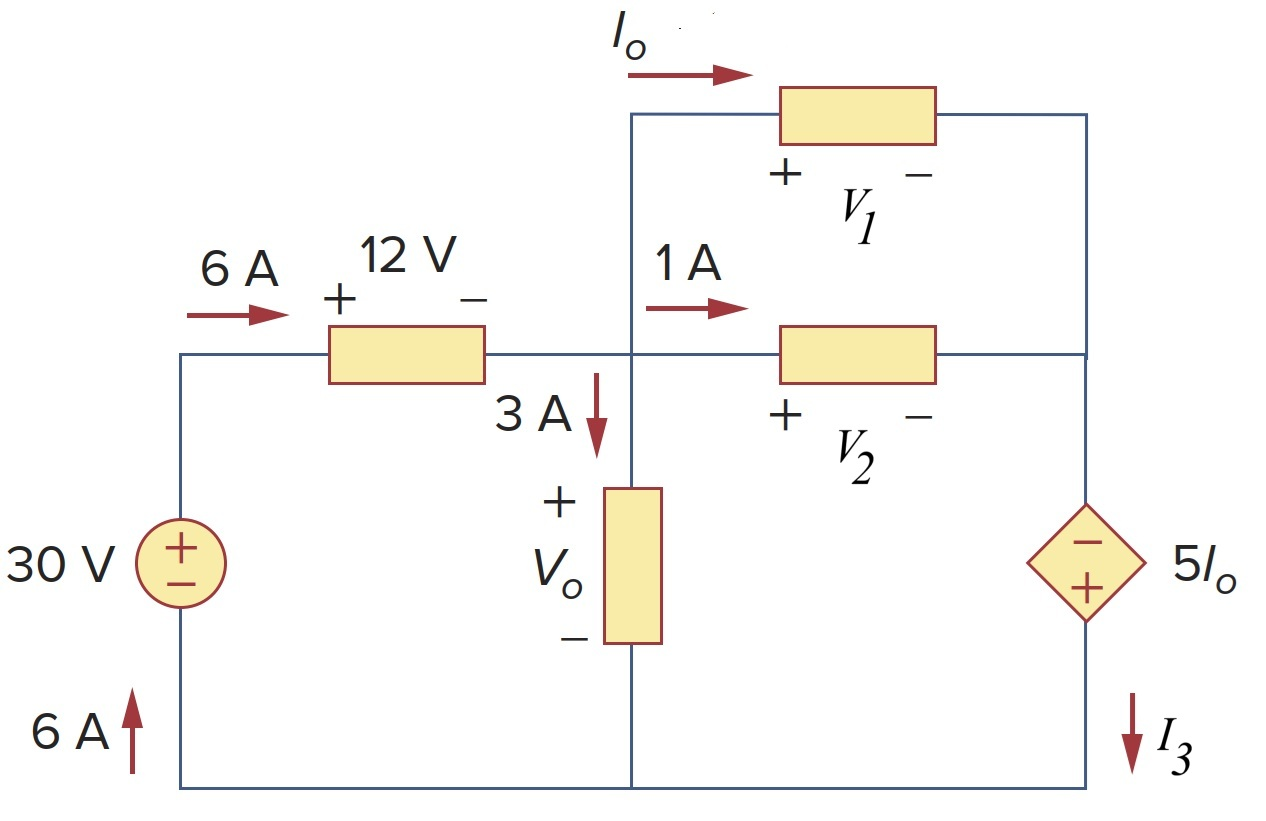
\includegraphics[width=0.5\textwidth]{fig_pw_kvcl.jpg}
	\caption{Circuit for Problem~\ref{pb:p3}.}
	\label{fig_1_31}
\end{figure}


\noindent\makebox[\linewidth]{\color{rouge_poly}{\rule{\textwidth}{1.3pt}}}

\begin{solprob} \text{}\\
    To start, it is important to note Kirchoff's Current Law ($I_\text{in} = I_\text{out}$) (KCL) and Kirchoff's Voltage Law ($\Sigma V_\text{loop} = 0$) (KVL).  First, we will apply KCL to solve for $I_o$.

    \begin{gather}
    I_\text{in} = I_\text{out}\\
    6A = 3A + 1A + I_o\\
    I_o = 6A-4A = 2A
    \end{gather}
    With this, I can use KCL again to solve for $I_3$.
    \begin{gather}
        I_o + 1A = I_3\\
        I_3 = (2A) + 1A = 3A
    \end{gather}

    With this information, we can calculate the voltage of the dependent voltage source in the bottom right corner of the circuit.
    \begin{gather}
        5I_o = 5(2A) = 10V
    \end{gather}

    Now, we have solved for all of the missing currents; we just need to solve for the voltages using KVL.  I am going to begin by using the mesh in the lower left-hand side of the circuit.
    \begin{gather}
        30V-12V-V_o = 0\\
        18V-V_o = 0
        V_o = 18V
    \end{gather}

    Now, I apply KVL again on the lower right-hand mesh to solve for $V_2$.
    \begin{gather}
        10V + 18V - V_2 = 0\\
        V_2 = 10V + 18V\\
        V_2 = 28V
    \end{gather}
    Lastly, I will select the entire right-side loop of the circuit and discard the left side, and apply KVL, ignoring any internal elements.
    \begin{gather}
        10V + 18V-V_1 = 0\\
        V_1 = 10V + 18V\\
        V_1 = 28V
    \end{gather}

    So, my final values are: \[
    I_o = 3A, \, I_3 = 3A, \, V_o = 18V, \, V_1 = 28V, \, V_2 = 28V
    \]
\end{solprob}

\noindent\makebox[\linewidth]{\color{rouge_poly}{\rule{\textwidth}{1.3pt}}}	
%%%%%%%%%%%%%%%%%%%%%%%%%%%%%%%%%%%%%%%%%%%%%%%%%%%%%%%%%%%%%%%%%%%%%%%%%%%%%%%%%%%%%%%%%%%%%%%%%%%%%%%%%%%%%%
%%%%%%%%%%%%%%%%%%%%%%%%%%%%%%%%%%%%%%%%%%%%%%%%%%%%%%%%%%%%%%%%%%%%%%%%%%%%%%%%%%%%%%%%%%%%%%%%%%%%%%%%%%%%%%
%%%%%%%%%%%%%%%%%%%%%%%%%%%%%%%%%%%%%%%%%%%%%%%%%%%%%%%%%%%%%%%%%%%%%%%%%%%%%%%%%%%%%%%%%%%%%%%%%%%%%%%%%%%%%%
%%%%%%%%%%%%%%%%%%%%%%%%%%%%%%%%%%%%%%%%%%%%%%%%%%%%%%%%%%%%%%%%%%%%%%%%%%%%%%%%%%%%%%%%%%%%%%%%%%%%%%%%%%%%%%

\begin{prob}\label{pb:p4}
	The voltage and current at the terminals of the circuit element in Fig.~\ref{fig_1_5} are zero for $t<0$. For $t\ge 0$, they are
	\[
	v(t)=100e^{-500t}\ \mathrm{V},\qquad
	i(t)=20-20e^{-500t}\ \mathrm{mA}.
	\]
	\begin{enumerate}[label=(\alph*)]
		\item Find the maximum value of the power delivered to the circuit.
		\item Find the total energy delivered to the element.
		\item Plot the power and energy signals, and verify your answers using MATLAB/Simulink or PSpice.
	\end{enumerate}
\end{prob}

\begin{figure}[H]
	\centering
	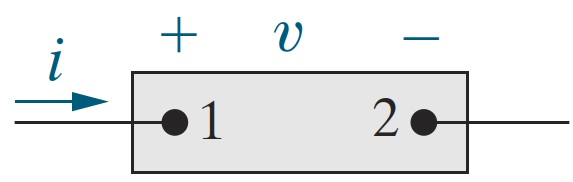
\includegraphics[width=0.25\textwidth]{fig_gen_elem.jpg}
	\caption{An ideal basic circuit element.}
	\label{fig_1_5}
\end{figure}


\noindent\makebox[\linewidth]{\color{rouge_poly}{\rule{\textwidth}{1.3pt}}}

\begin{solprob} \text{}\\
    (a)\[v(t) = 100e^\text{500t} V \,\,\,\,\,\,\, i(t) = 20 - 20e^\text{-500t} mA\]
    Solving for p(t):
    \[p(t) = v(t)i(t) = 100e^\text{500t}(20 - 20e^\text{-500t}) mW\]
    Simplifying and converting mW to W:
    \[p(t) = 2e^\text{-500t}-2e^\text{-1000t} W\]
    To find the maximum time, we need to find the critical point of p(t):
    \[\frac{dp}{dt} = -1000e^\text{-500t} + 2000e^{-1000t} = 0\]
    \[1000e^\text{-500t} = 2000e^\text{-1000t}\]
    \[e^\text{500t} = 2\]
    \[500t = \ln(2)\]
    \[t_\text{max} = \frac{\ln(2)}{500} \approx 0.001386\text{s} = 1.386 \text{ms}\]
    Subbing $t_\text{max}$ back into p(t):
    \begin{align}
        p(0.001386) & = 2e^\text{-500(0.001386)}-2e^\text{-1000(0.001386)}\\
        & = 2e^\text{-0.69}-2e^\text{-1.386}\\
        & = 1- \frac{1}{2}\\
        & = 0.5\,W
    \end{align}
    (b)
    \begin{align}
        W\text{(Energy)} & = \int_0^\text{$t_\text{max}$} p(t) \, dt = \int_0^\text{$t_\text{max}$} 2e^\text{-500t}-2e^\text{-1000t}\,dt\\
        & = 2(\frac{-e^\text{-500($\infty$)}}{500} + \frac{e^\text{-1000($\infty$)}}{1000}) - 2(\frac{-e^\text{-500(0)}}{500} + \frac{e^\text{-1000(0)}}{1000})\\
        & = (\frac{0}{250} + \frac{0}{500}) - (\frac{-1}{250} + \frac{1}{500})\\
        & = 2 \text{mJ}
    \end{align}
    (c)
    \begin{figure}[H]
    	\centering
    	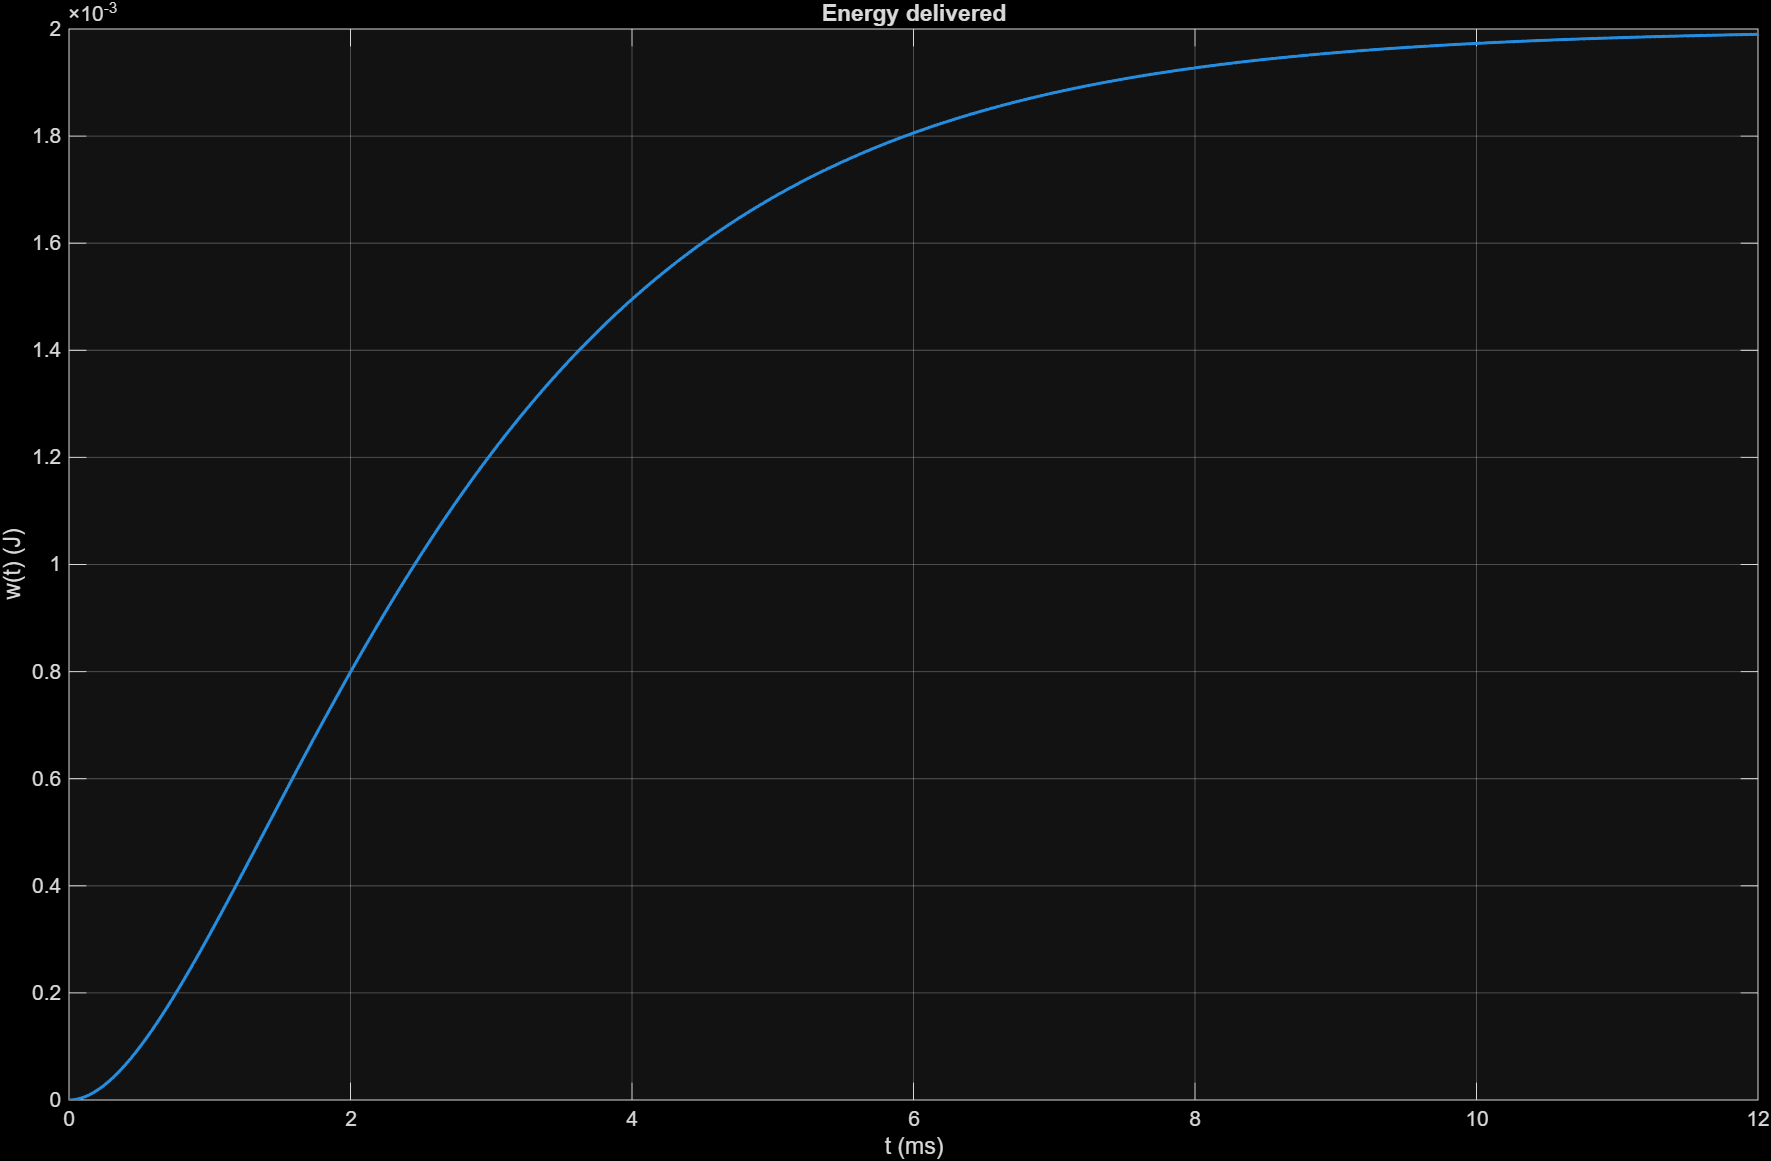
\includegraphics[width=0.75\textwidth]{EECS2200 - Homework1- 4c.png}
    	\caption{Energy Delivered over time}
    	\label{fig_1_5}
    \end{figure}

    \begin{figure}[H]
    	\centering
    	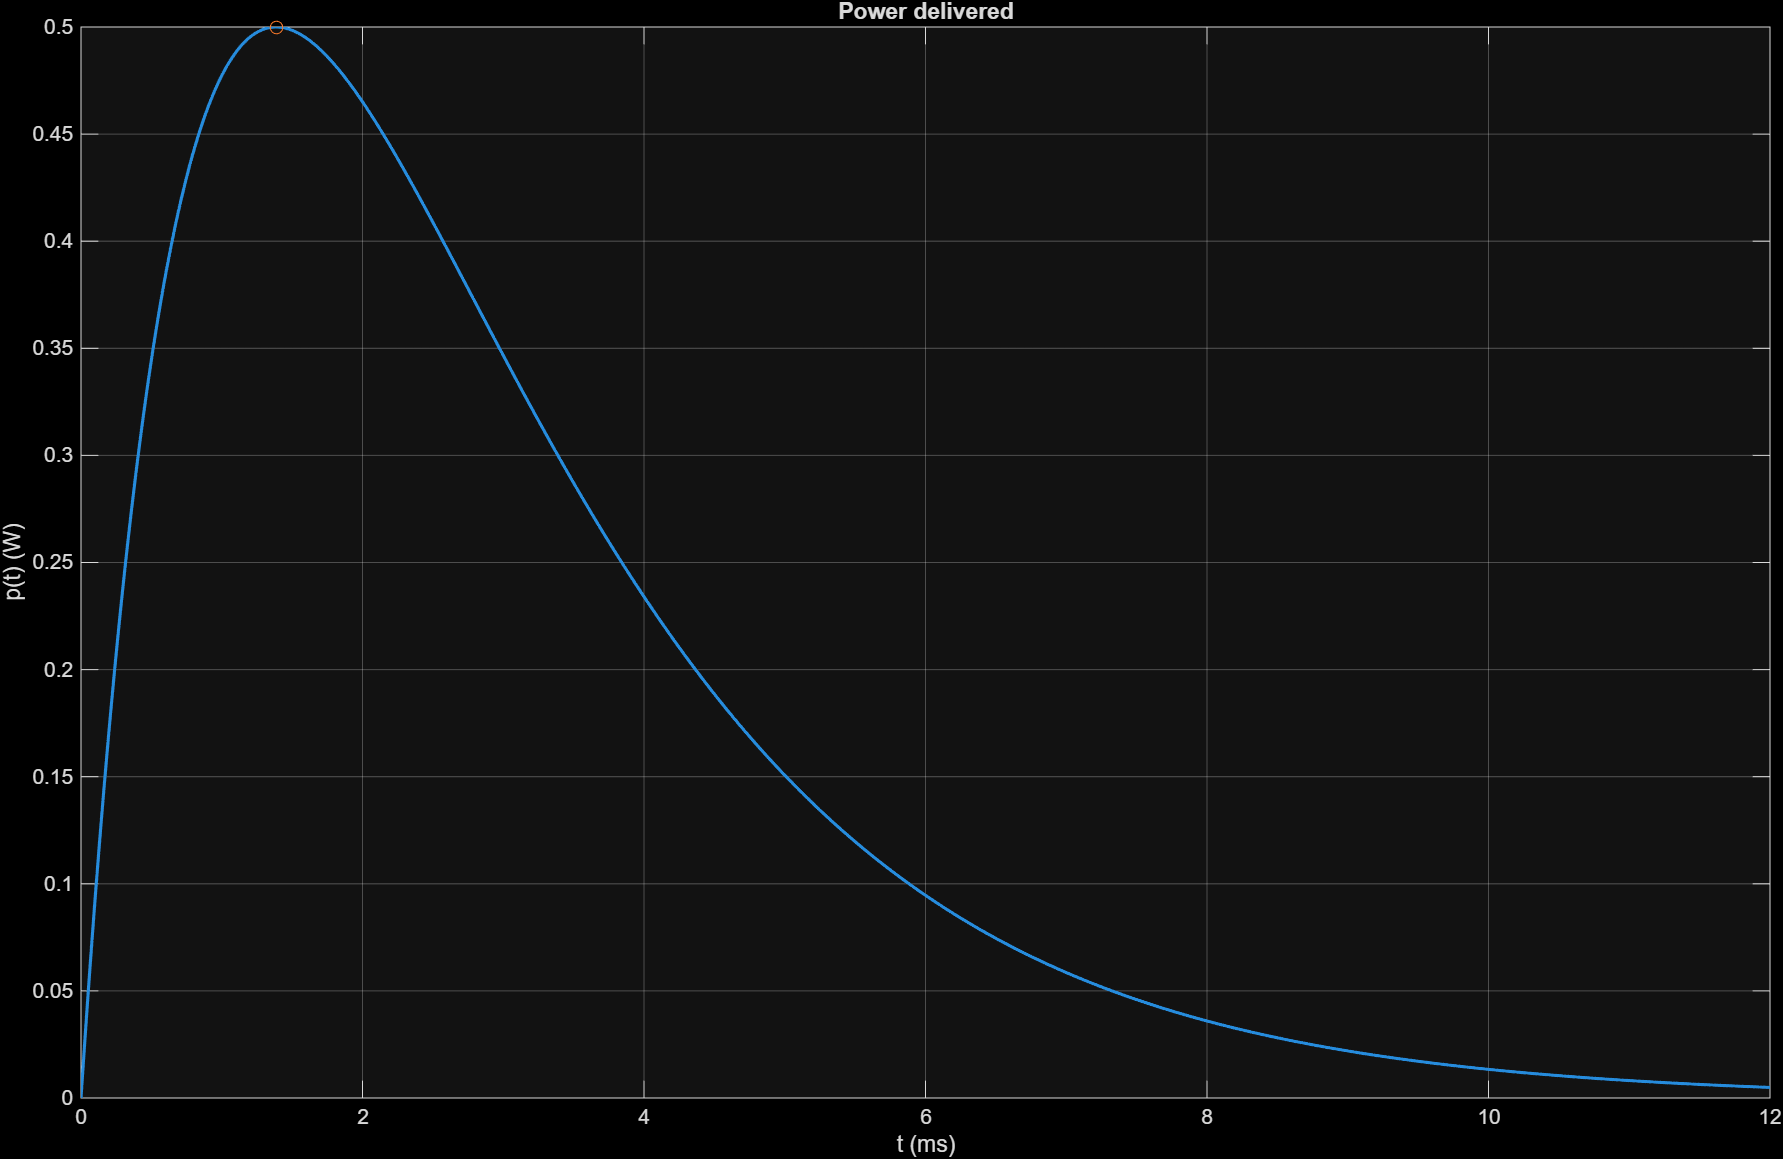
\includegraphics[width=0.75\textwidth]{EECS2200 - Homework1- 4c2.png}
    	\caption{Power delivered over time}
    	\label{fig_1_5}
    \end{figure}
    
\end{solprob}

\noindent\makebox[\linewidth]{\color{rouge_poly}{\rule{\textwidth}{1.3pt}}}	
%%%%%%%%%%%%%%%%%%%%%%%%%%%%%%%%%%%%%%%%%%%%%%%%%%%%%%%%%%%%%%%%%%%%%%%%%%%%%%%%%%%%%%%%%%%%%%%%%%%%%%%%%%%%%%
%%%%%%%%%%%%%%%%%%%%%%%%%%%%%%%%%%%%%%%%%%%%%%%%%%%%%%%%%%%%%%%%%%%%%%%%%%%%%%%%%%%%%%%%%%%%%%%%%%%%%%%%%%%%%%
%%%%%%%%%%%%%%%%%%%%%%%%%%%%%%%%%%%%%%%%%%%%%%%%%%%%%%%%%%%%%%%%%%%%%%%%%%%%%%%%%%%%%%%%%%%%%%%%%%%%%%%%%%%%%%
%%%%%%%%%%%%%%%%%%%%%%%%%%%%%%%%%%%%%%%%%%%%%%%%%%%%%%%%%%%%%%%%%%%%%%%%%%%%%%%%%%%%%%%%%%%%%%%%%%%%%%%%%%%%%%

\begin{prob}\label{pb:p5}
	The voltage and current at the terminals of the circuit element in Fig.~\ref{fig_1_5} are zero for $t<0$ and $t>3\ \mathrm{s}$. In the interval $0<t<3\ \mathrm{s}$ the expressions are
	\[
	v(t)=t(3-t)\ \mathrm{V},\qquad 0<t<3\ \mathrm{s},
	\]
	\[
	i(t)=(6-4t)\ \mathrm{mA},\qquad 0<t<3\ \mathrm{s}.
	\]
\begin{enumerate}[label=(\alph*)]
	\item Determine the instant of time when the power delivered to the circuit element is maximum and compute the corresponding power.
	\item Determine the instant of time when the power extracted from the circuit element is maximum and compute the corresponding power.
	\item Calculate the net energy delivered to the circuit at $t=0,\ 1,\ 2,$ and $3\ \mathrm{s}$.
\end{enumerate}
\end{prob}



\noindent\makebox[\linewidth]{\color{rouge_poly}{\rule{\textwidth}{1.3pt}}}

\begin{solprob} \text{}\\
    We begin with the first two initial equations: $V(t) = t(3-t)$ and $i(t) = 6-4t$.  The first step is to combine the initial equations to calculate power over time.
    \[p(t) = v(t)i(t) = t(3-t)(6-4t) = t(18-18t+4t^2) = 18t-18t^2+4t^3\]
    Now, we find the derivative of the expanded power equation and solve for its roots.
    \[p^\prime = 18-36t+12t^2 = 0\]
    Now, lets use the quadratic formula to solve for the roots of the derivative.
    \[t = \frac{-b\pm \sqrt{b^2 - 4ac}}{2a} = \frac{-(-36)\pm \sqrt{(-36)^2 - 4(12)(18)}}{2(12)}\]
    \[t = \frac{36 \pm \sqrt{432}}{24}\]
    Now, solving for t, we get 2 roots: $t_ 1 = 2.366$s and $t_2 = 0.6339$s. To figure out which one is the maximum power delivered or extracted, we need to plug $t_1$ and $t_2$ back into the power equation.
    \[p(t_1) = p(2.366) = 2.366(3-2.366)(6-4(2.366)) = -5.19mW\text{(}\]
    \[p(t_2) = p(0.6339) = 0.6339(3-0.6339)(6-4(0.6339)) = 5.19mW\]
    $\therefore$ (a)the maximum power delivered is 5.19 mW and it happens at 2.366s and (b) the maximum power extracted is 5.19 mW and it happens at 0.6339s.
    \\(c)\\
    To calculate the net energy delivered, we can immediately rule out two of the values due to the graphs symmetry. Because t=0 and t=3 are both roots and have opposite behaviour, so their net energy cancels each other out resulting in a net power of zero.\\
    To continue to calculate the net power at 1s and 2s, we need to find the integral of the power function.
    \[W = \int_0^tp(t)\,dt\]
    \[W_\text{net(1)} = \int_0^1 18t-18t^2+4t^3\,dt = 9t^2-6t^3 + t^4|_0^1\]
    \[W_\text{net(1)} = 9(1)^2 - 6(1)^3+(1)^4 = 9-6+1 = 4mW(net)\]
    Now, because we still know this function is symmetrical on 0 < t < 3, the change from 1s to 2s will not actually affect the net value, and effectively cancel out, so net energy at 2s is also 4mW.
    
\end{solprob}

\noindent\makebox[\linewidth]{\color{rouge_poly}{\rule{\textwidth}{1.3pt}}}	
%%%%%%%%%%%%%%%%%%%%%%%%%%%%%%%%%%%%%%%%%%%%%%%%%%%%%%%%%%%%%%%%%%%%%%%%%%%%%%%%%%%%%%%%%%%%%%%%%%%%%%%%%%%%%%
%%%%%%%%%%%%%%%%%%%%%%%%%%%%%%%%%%%%%%%%%%%%%%%%%%%%%%%%%%%%%%%%%%%%%%%%%%%%%%%%%%%%%%%%%%%%%%%%%%%%%%%%%%%%%%
%%%%%%%%%%%%%%%%%%%%%%%%%%%%%%%%%%%%%%%%%%%%%%%%%%%%%%%%%%%%%%%%%%%%%%%%%%%%%%%%%%%%%%%%%%%%%%%%%%%%%%%%%%%%%%
%%%%%%%%%%%%%%%%%%%%%%%%%%%%%%%%%%%%%%%%%%%%%%%%%%%%%%%%%%%%%%%%%%%%%%%%%%%%%%%%%%%%%%%%%%%%%%%%%%%%%%%%%%%%%%

\begin{prob}\label{pb:p6}
	The numerical values of the voltages and currents in the electrical network of Fig.~\ref{fig:P_check} are given in Table~\ref{tab:P1_31}. Does the network satisfy the power balance?
\end{prob}

\begin{figure}[H]
	\centering
	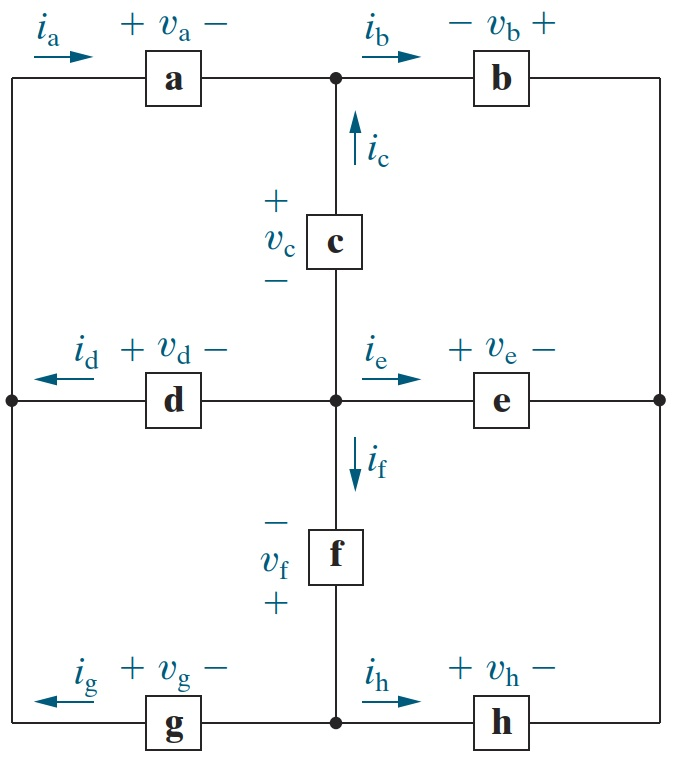
\includegraphics[width=0.5\textwidth]{fig_P_check.jpg}
	\caption{Electrical network for Problem~\ref{pb:p6}.}
	\label{fig:P_check}
\end{figure}

\begin{table}[H]
	\centering
	\caption{Voltages and currents of the elements.}
	\label{tab:P1_31}
	\begin{tabular}{c r r}
		\hline
		Element & Voltage (V) & Current (mA) \\ \hline
		a & 6   & 500  \\
		b & 10  & 100  \\
		c & -8  & -400 \\
		d & -2  & 300  \\
		e & -2  & 300  \\
		f & 4   & -200 \\
		g & -6  & 200  \\
		h & 2   & -400 \\
		\hline
	\end{tabular}
\end{table}


\noindent\makebox[\linewidth]{\color{rouge_poly}{\rule{\textwidth}{1.3pt}}}

\begin{solprob} \text{}\\
    To calculate power balance, we should calculate power at each element and then sum them all together.
    
    \[p_a = v_ai_a=(6\text{V})(500\text{mA}) = 3000\text{mW} = 3\text{W}\]
    \[p_b= -v_bi_b = -(10\text{V})(100\text{mA}) = -1000\text{mW} = -1\text{W}\]
    \[p_c= -v_ci_c=-(-8\text{V})(-400\text{mA}) = -3200\text{mW} = -3.2\text{W}\]
    \[p_d = -v_di_d = -(-2\text{V})(300\text{mA}) = 600\text{mW} = 0.6\text{W}\]
    \[p_e = v_ei_e = (-2\text{V})(300\text{mA}) = -600\text{mW} = -0.6\text{W}\]
    \[p_f = -v_fi_f = -(4\text{V})(-200\text{mA}) = 800\text{mW} = 0.8\text{W}\]
    \[p_g = -v_gi_g = -(-6\text{V})(200\text{mA}) = 1200\text{mW} = 1.2\text{W}\]
    \[p_h = v_hi_h = (2\text{V})(-400\text{mA}) = -800\text{mW} = -0.8\text{W}\]
    \[\]
    \begin{align}
        p_\text{total} & = 3\text{W} - 1\text{W} -3.2\text{W} + 0.6\text{W}-0.6\text{W}+0.8\text{W}+1.2\text{W}-0.8\text{W}\\
        & = 0\text{W} \therefore \text{power balances}
    \end{align}
\end{solprob}

\noindent\makebox[\linewidth]{\color{rouge_poly}{\rule{\textwidth}{1.3pt}}}	
%%%%%%%%%%%%%%%%%%%%%%%%%%%%%%%%%%%%%%%%%%%%%%%%%%%%%%%%%%%%%%%%%%%%%%%%%%%%%%%%%%%%%%%%%%%%%%%%%%%%%%%%%%%%%%
%%%%%%%%%%%%%%%%%%%%%%%%%%%%%%%%%%%%%%%%%%%%%%%%%%%%%%%%%%%%%%%%%%%%%%%%%%%%%%%%%%%%%%%%%%%%%%%%%%%%%%%%%%%%%%
%%%%%%%%%%%%%%%%%%%%%%%%%%%%%%%%%%%%%%%%%%%%%%%%%%%%%%%%%%%%%%%%%%%%%%%%%%%%%%%%%%%%%%%%%%%%%%%%%%%%%%%%%%%%%%
%%%%%%%%%%%%%%%%%%%%%%%%%%%%%%%%%%%%%%%%%%%%%%%%%%%%%%%%%%%%%%%%%%%%%%%%%%%%%%%%%%%%%%%%%%%%%%%%%%%%%%%%%%%%%%

\begin{prob}\label{pb:p7}
	If the interconnection in Fig.~\ref{fig:cir_valid} is valid, find the total power developed in the circuit. If the interconnection is not valid, explain why.
\end{prob}

\begin{figure}[H]
	\centering
	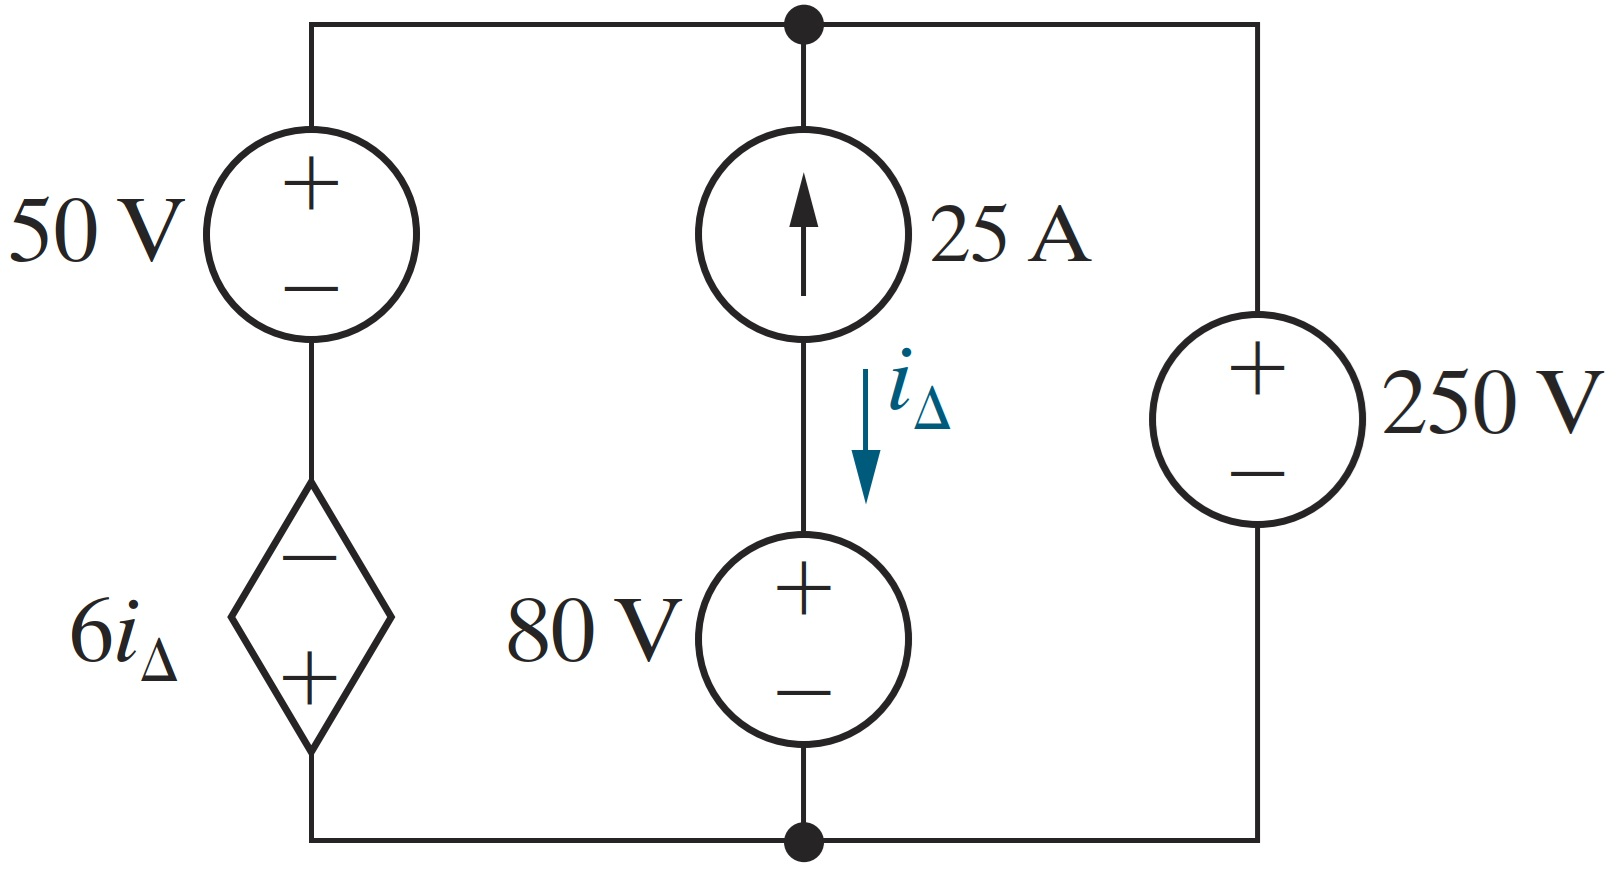
\includegraphics[width=0.5\textwidth]{fig_cir_valid1.jpg}
	\caption{Circuit interconnection for Problem~\ref{pb:p7}.}
	\label{fig:cir_valid}
\end{figure}

\noindent\makebox[\linewidth]{\color{rouge_poly}{\rule{\textwidth}{1.3pt}}}

\begin{solprob} \text{}\\
    To begin the problem, we do KVL around the entire outer wire of the loop.
    \[-6i_\Delta + 50V - 250V = 0\]
    Now let's solve for $i_\Delta$:
    \[-6i_\Delta = 250V-50V\]
    \[i_\Delta = \frac{-200}{6}\]
    \[i_\Delta \approx -33.33\]
    $\therefore$ The interconnection is not possible because the current on the middle wire would technically have 2 different currents (which is not possible because current is constant throughout a series circuit).  This can be seen because the current source is providing 25 A, but $I_\Delta$ is -33.33 A, which are not equal. $\therefore$ This interconnection is not possible.
\end{solprob}

\noindent\makebox[\linewidth]{\color{rouge_poly}{\rule{\textwidth}{1.3pt}}}	
%%%%%%%%%%%%%%%%%%%%%%%%%%%%%%%%%%%%%%%%%%%%%%%%%%%%%%%%%%%%%%%%%%%%%%%%%%%%%%%%%%%%%%%%%%%%%%%%%%%%%%%%%%%%%%
%%%%%%%%%%%%%%%%%%%%%%%%%%%%%%%%%%%%%%%%%%%%%%%%%%%%%%%%%%%%%%%%%%%%%%%%%%%%%%%%%%%%%%%%%%%%%%%%%%%%%%%%%%%%%%
%%%%%%%%%%%%%%%%%%%%%%%%%%%%%%%%%%%%%%%%%%%%%%%%%%%%%%%%%%%%%%%%%%%%%%%%%%%%%%%%%%%%%%%%%%%%%%%%%%%%%%%%%%%%%%
%%%%%%%%%%%%%%%%%%%%%%%%%%%%%%%%%%%%%%%%%%%%%%%%%%%%%%%%%%%%%%%%%%%%%%%%%%%%%%%%%%%%%%%%%%%%%%%%%%%%%%%%%%%%%%

\begin{prob}\label{pb:p8}
	For the circuit shown in Fig.~\ref{fig:amp2}:  
	\begin{enumerate}[label=(\alph*)]
		\item Calculate $i_\Delta$ and $v_o$.
		\item Show that the power developed equals the power absorbed.
	\end{enumerate}
\end{prob}

\begin{figure}[htbp]
	\centering
	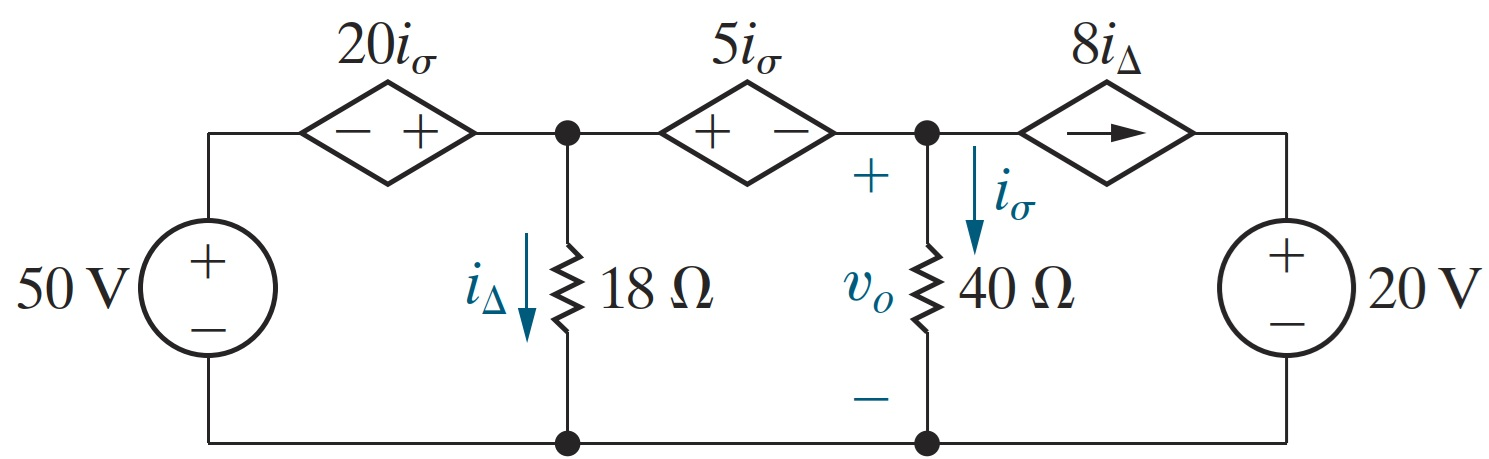
\includegraphics[width=0.7\textwidth]{fig_amp2.jpg}
	\caption{Circuit for Problem~\ref{pb:p8}.}
	\label{fig:amp2}
\end{figure}




\noindent\makebox[\linewidth]{\color{rouge_poly}{\rule{\textwidth}{1.3pt}}}

\begin{solprob} \text{}\\
    (a) Let's begin by using KVL on the loop containing the left and middle meshes.
    \begin{gather}
        50 + 20i_\sigma - 5i_\sigma - 40i_\sigma = 0\\
        i_\sigma(-20 + 5 + 40) = 50\\
        i_\sigma=\frac{50}{25} = 2\text{A}
    \end{gather}

    Now, let's do KVL on the left-hand mesh to solve for $i_\Delta$
    \begin{gather}
        50 + 20i_\sigma - 18i_\Delta = 0\\
        50 + 20(2) = 18i_\Delta\\
        i_\Delta = \frac{90}{18} = 5\text{A}
    \end{gather}
    Finally, let's use Ohm's law on the $40\Omega$ resistor to get $v_o$.
    \begin{gather}
        V = IR \Rrightarrow v_o = I_\sigma(40\Omega) = 2\text{A}(40\Omega) = 80\text{V}
    \end{gather}

    (b)
    Let's begin by using KCL to solve for some unknown current values.
    \[I_\text{$5i_\sigma$} = i_\sigma + 8i_\Delta = 2\text{A} + 8\text{A}(5\text{A}) = 42\text{A}\]
    We also need to solve for $i_\text{50}$ and $i_\text{$20i_\sigma$}$.
    \[I_\text{$20i_\sigma$} = i_\Delta + I_\text{$5i_\sigma$} = 5\text{A} + 42\text{A} = 47\text{A}\]
    Because these elements are in series with each other, they share the same current, so $I_\text{50} = I_\text{$20i_\sigma$}$. Before we begin solving for power balance, we must also solve for $V_\text{$8i_\Delta$}$. We can do this by taking the potential difference between two wires in parallel.
    \[V_\text{$8i_\Delta$} = V_o - 20\text{V} = 80\text{V} - 20\text{V} = 60\text{V}\]
    For simplicity, we will calculate the power from the voltage and current sources, as well as the resistors individually.
    \[p_\text{vs} = -50(47)-20(2)(47) + 5(2)(42) + 20(8)(5) = -3010 \text{ W}\]
    \[p_R = 18i^2_\Delta + 40i^2_\sigma = 18(5)^2 + 40(2)^2 = 610 \text{ W}\]
    \[p_\text{cs} = v_\text{$8i_\Delta$}(8i_\Delta) = 60(40) = 2400 \text{ W}\]
    \[P_\text{total} = p_\text{vs} + p_\text{cs} + p_R = -3010 + 2400 + 610 = 0\text{ W} \therefore \text{power balances}\]
\end{solprob}

\noindent\makebox[\linewidth]{\color{rouge_poly}{\rule{\textwidth}{1.3pt}}}	
%%%%%%%%%%%%%%%%%%%%%%%%%%%%%%%%%%%%%%%%%%%%%%%%%%%%%%%%%%%%%%%%%%%%%%%%%%%%%%%%%%%%%%%%%%%%%%%%%%%%%%%%%%%%%%
%%%%%%%%%%%%%%%%%%%%%%%%%%%%%%%%%%%%%%%%%%%%%%%%%%%%%%%%%%%%%%%%%%%%%%%%%%%%%%%%%%%%%%%%%%%%%%%%%%%%%%%%%%%%%%
%%%%%%%%%%%%%%%%%%%%%%%%%%%%%%%%%%%%%%%%%%%%%%%%%%%%%%%%%%%%%%%%%%%%%%%%%%%%%%%%%%%%%%%%%%%%%%%%%%%%%%%%%%%%%%
%%%%%%%%%%%%%%%%%%%%%%%%%%%%%%%%%%%%%%%%%%%%%%%%%%%%%%%%%%%%%%%%%%%%%%%%%%%%%%%%%%%%%%%%%%%%%%%%%%%%%%%%%%%%%%

\begin{prob}\label{pb:p9}
	Find $v_1$ and $v_g$ in the circuit shown in Fig.~\ref{fig:amp1} when $v_o = 250\ \mathrm{mV}$. 
	(Hint: Start at the right end of the circuit and work back toward $v_g$.)
\end{prob}

\begin{figure}[H]
	\centering
	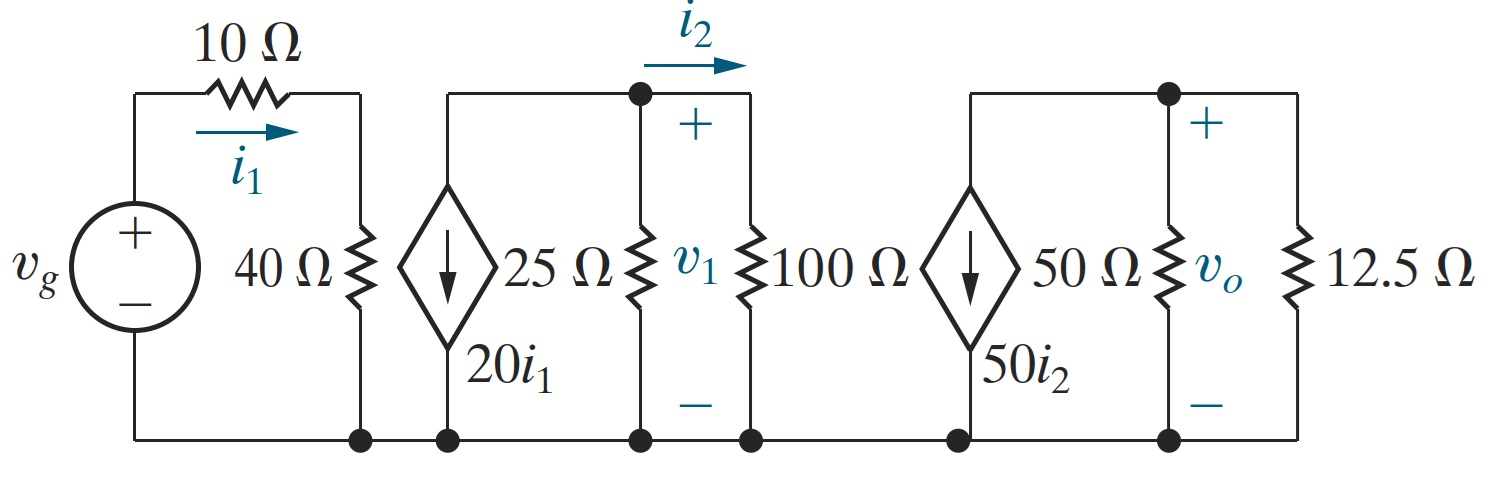
\includegraphics[width=0.7\textwidth]{fig_amp1.jpg}
	\caption{Circuit for Problem~\ref{pb:p9}.}
	\label{fig:amp1}
\end{figure}


\noindent\makebox[\linewidth]{\color{rouge_poly}{\rule{\textwidth}{1.3pt}}}

\begin{solprob} \text{}\\
    To begin, we use nodal analysis on the node right below $50i_2$ to solve for $i_2$.
    \[i_2 = \frac{v_o}{50} + \frac{v_o}{12.5} + 50i_2\]
    \[-49i_2 = \frac{0.25}{50} + \frac{0.25}{12.5}\]
    \[i_2 = -0.510\text{ mA}\]
    Now, by knowing parallel circuits, we can determine that $v_1$ is actually equivalent to $v_o$. So:
    \[v_1 = v_o = 250\text{mV}\]
    Before we can move forward, we need to figure out what $v_1$ is.  Now, we use nodal analysis on the far left node below the $40\Omega$ resistor.
    \[i_1 = \frac{v_1}{40} + \frac{v_1}{25} + \frac{v_1}{100} + 20i_1 + i_2\]
    \[i_1 = v_1(\frac{1}{40} + \frac{1}{25} + \frac{1}{100}) + (-0.510)\]
    \[i_1 = -0.96\text{mA}\]
    Now, we can find $v_g$ using this equation:
    \[v_1 = v_g - 10i_1\]
    \[v_g = 0.25 + 10(-0.96mA) = 0.240V\]
    \[\therefore \text{$v_1 = 250$mV and $V_g \approx 240$mV}\]
\end{solprob}

\noindent\makebox[\linewidth]{\color{rouge_poly}{\rule{\textwidth}{1.3pt}}}	
%%%%%%%%%%%%%%%%%%%%%%%%%%%%%%%%%%%%%%%%%%%%%%%%%%%%%%%%%%%%%%%%%%%%%%%%%%%%%%%%%%%%%%%%%%%%%%%%%%%%%%%%%%%%%%
%%%%%%%%%%%%%%%%%%%%%%%%%%%%%%%%%%%%%%%%%%%%%%%%%%%%%%%%%%%%%%%%%%%%%%%%%%%%%%%%%%%%%%%%%%%%%%%%%%%%%%%%%%%%%%
%%%%%%%%%%%%%%%%%%%%%%%%%%%%%%%%%%%%%%%%%%%%%%%%%%%%%%%%%%%%%%%%%%%%%%%%%%%%%%%%%%%%%%%%%%%%%%%%%%%%%%%%%%%%%%
%%%%%%%%%%%%%%%%%%%%%%%%%%%%%%%%%%%%%%%%%%%%%%%%%%%%%%%%%%%%%%%%%%%%%%%%%%%%%%%%%%%%%%%%%%%%%%%%%%%%%%%%%%%%%%

\begin{prob}\label{pb:p10}
	For the circuit shown in Fig.~\ref{fig:amp3}, find the current $i_1$ in microamperes, the voltage $v$ in volts, the total power generated, and the total power absorbed.
\end{prob}

\begin{figure}[H]
	\centering
	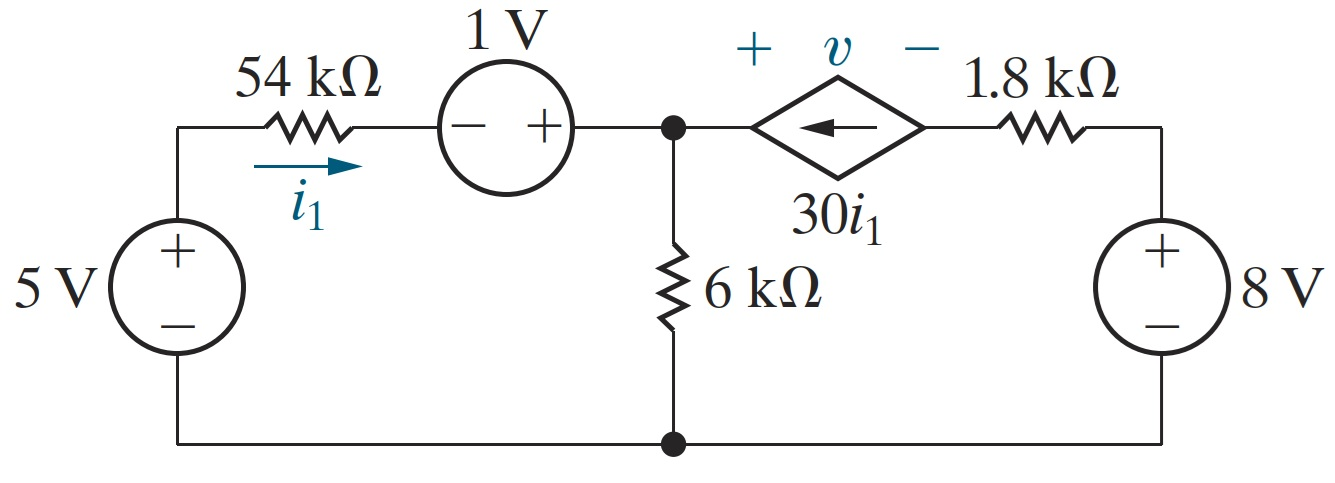
\includegraphics[width=0.6\textwidth]{fig_amp3.jpg}
	\caption{Circuit for Problem~\ref{pb:p10}.}
	\label{fig:amp3}
\end{figure}



\noindent\makebox[\linewidth]{\color{rouge_poly}{\rule{\textwidth}{1.3pt}}}

\begin{solprob} \text{}\\
    Let's begin by using KVL on the left mesh.
    \[5-54000i_1 + 1 - 6000i_6 = 0\]
    Now, let's do KCL on the top node.
    \[i_1 + 30i_1 = i_6 = 31i_1\]
    Substituting $i_6$ back into the KVL above:
    \[6-54000i_1-6000(31i_1) = 0\]
    \[6-54000i_1-186000i_1=0\]
    \[i_1 = 25\text{$\mu$V}\]

    Subbing $i_1$ back into the KCL to solve for $i_6$.

    \[i_6 = 31(25\mu V)\]

    Now, lets do KVL on the right mesh.

    \[-8 + 6000i_6 - v + 1800(30i_1) = 0\]
    Solving for $v$:
    \begin{align}
        v & = 6000i_6 + 54000i_1 - 8\\
        & = 6000(775 \mu) + 54000(25 \mu) - 8 = -2\text{V}
    \end{align}

    Now, we move towards finding the power generated and absorbed. We start by finding the power generated or absorbed in all the elements.

    \[p_\text{5V} = -vi = -(5)(25\mu) = -125\mu W\]
    \[p_\text{54k} = RI^2 = 54000(25\mu)^2 \approx 33.75\mu W\]
    \[p_\text{1V} = -vi = -(1)(25\mu) = -25\mu W\]
    \[p_\text{6k} = RI^2 = 6000(775\mu)^2 \approx 3603\mu W\]
    \[p_\text{cs} = vi = (2)(750\mu) = 1500\mu W\]
    \[p_\text{1.8k} = RI^2 =  1800(750\mu)^2 \approx 1012.5\mu W\]
    \[p_\text{8V} = -vi = -(8)(750\mu) \approx -6000\mu W\]
    \[p_\text{total} = -125\mu W + 33.75\mu W -25\mu W + 3603\mu W + 1500\mu W + 1012.5\mu W -6000\mu W = 0\]
    \[\therefore \text{power balances!}\]
    
\end{solprob}

\noindent\makebox[\linewidth]{\color{rouge_poly}{\rule{\textwidth}{1.3pt}}}	
%%%%%%%%%%%%%%%%%%%%%%%%%%%%%%%%%%%%%%%%%%%%%%%%%%%%%%%%%%%%%%%%%%%%%%%%%%%%%%%%%%%%%%%%%%%%%%%%%%%%%%%%%%%%%%
%%%%%%%%%%%%%%%%%%%%%%%%%%%%%%%%%%%%%%%%%%%%%%%%%%%%%%%%%%%%%%%%%%%%%%%%%%%%%%%%%%%%%%%%%%%%%%%%%%%%%%%%%%%%%%
%%%%%%%%%%%%%%%%%%%%%%%%%%%%%%%%%%%%%%%%%%%%%%%%%%%%%%%%%%%%%%%%%%%%%%%%%%%%%%%%%%%%%%%%%%%%%%%%%%%%%%%%%%%%%%
%%%%%%%%%%%%%%%%%%%%%%%%%%%%%%%%%%%%%%%%%%%%%%%%%%%%%%%%%%%%%%%%%%%%%%%%%%%%%%%%%%%%%%%%%%%%%%%%%%%%%%%%%%%%%%
\hfill \break
\begin{prob}\label{pb:p11}

	The currents $i_1$ and $i_2$ in the circuit in Fig.~\ref{fig:cir_res1} are 10 A and 25 A, respectively.  
	\begin{enumerate}[label=(\alph*)]
		\item Find the power supplied by each voltage source.
		\item Show that the total power supplied equals the total power dissipated in the resistors.
	\end{enumerate}
\end{prob}

\begin{figure}[H]
	\centering
	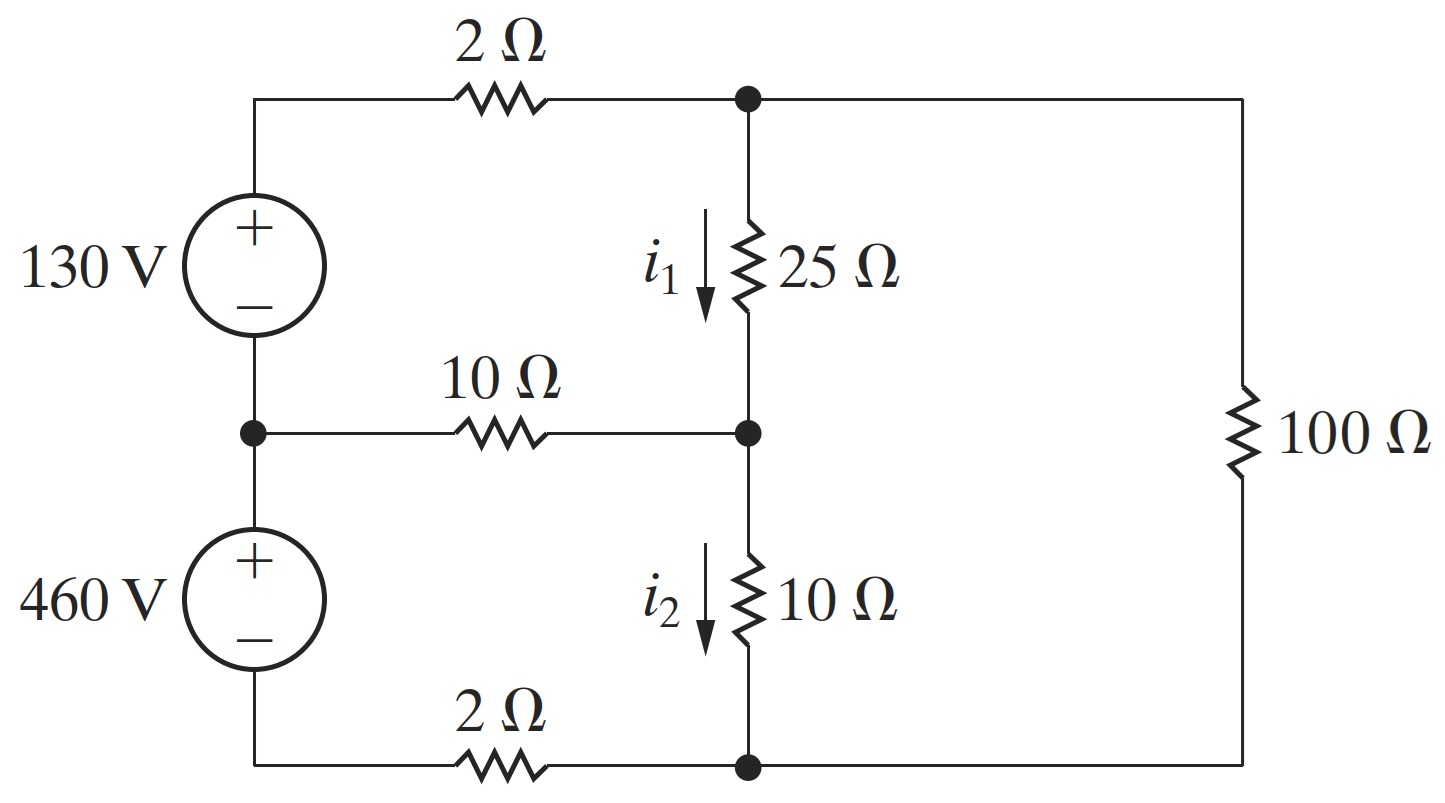
\includegraphics[width=0.5\textwidth]{fig_cir_res1.jpg}
	\caption{Circuit for Problem~\ref{pb:p11}.}
	\label{fig:cir_res1}
\end{figure}


\noindent\makebox[\linewidth]{\color{rouge_poly}{\rule{\textwidth}{1.3pt}}}

\begin{solprob} \text{}\\
    Lets begin by getting KVL at the top right mesh.
    \[130 - 2\text{$i_\text{$2\Omega$}$} - 25i_1 + 10\text{$i_\text{$10\Omega$}$} = 0\]
    Now, lets get $i_\text{$10\Omega$}$ using a KCL in the middle node.
    \[i_1 + i_\text{$10\Omega$} = i_2\]
    \[i_\text{$10\Omega$} = i_2-i_1\]
    \[i_\text{$10\Omega$} = 25-10 = 15\text{A}\]
    Now, lets get KVL at the bottom:
    \[460 + 10\text{$i_\text{$10\Omega$}$} - 10i_2 - 2\text{$i_\text{$2\Omega_2$}$}\]
    Now lets isolate $2\text{$i_\text{$2\Omega$}$}$ in the first KVL equation.
    \[i_\text{$2\Omega$} = \frac{130-25i_1 + 10\text{$i_\text{$10\Omega$}$}}{2}\]
    \[i_\text{$2\Omega$} = \frac{130-25(10) + 10(15)}{2}\]
    \[i_\text{$2\Omega$} = 15\text{A}\]
    Now that we have $i_\text{$2\Omega$}$, we want to find $i_\text{$100\Omega$}$, so we take the KCL on the top node.
    \[i_\text{$2\Omega$} = i_1 + i_\text{$100\Omega$}\]
    \[i_\text{$100\Omega$} = i_\text{$2\Omega$} - i_1 = 15\text{A}-10\text{A} = 5\text{A}\]
    Lets use this value to solve for the 2nd 2$\Omega$ resistor ($i_\text{$2\Omega_\text{2}$}$) on the bottom using its KCL on the bottom.
    \[i_2 + i_\text{$100\Omega$} = i_\text{$2\Omega_\text{2}$}\]
    \[i_\text{$2\Omega_\text{2}$} = 25\text{A} + 5\text{A} = 30\text{A}\]
    (a)
    The power supplied by each voltage source is shown below.
    \[p_\text{130V} = -vi_\text{$2\Omega$} = -(130V)(15A) = -1950W = 1950 \text{W generated}\]
    \[p_\text{460V} = -vi_\text{$2\Omega_\text{2}$} = -(460V)(30A) = -13800W = 13800\text{W generated}\]
    \[p_\text{generated} = -13800 + (-1950) = -15750 \text{W}\]

    (b)
    Now, let's calculate the individual power that each element consumes.
    \[p_\text{2$\Omega$} = RI^2 = 2(15\text{A})^2 = 450 \text{ W}\]
    \[p_\text{$25\Omega$} = RI^2 = 25(10)^2 = 2500 \text{ W}\]
    \[p_\text{$i_2$} = RI^2 = 10(25)^2 = 6250 \text{ W}\]
    \[p_\text{$10\Omega$} = RI^2 = 10(15)^2 = 2250 \text{ W}\]
    \[p_\text{$100\Omega$} = RI^2 = 100(5)^2 = 2500 \text{ W}\]
    \[p_\text{$2\Omega_2$} = RI^2 = 2(30)^2 = 1800 \text{ W}\]
    \[p_\text{total} = 450 + 2500 + 6250 + 2250 + 2500 + 1800 - 15750 = 0 \text{ W} \therefore \text{power balances}\]
    
\end{solprob}

\noindent\makebox[\linewidth]{\color{rouge_poly}{\rule{\textwidth}{1.3pt}}}	
%%%%%%%%%%%%%%%%%%%%%%%%%%%%%%%%%%%%%%%%%%%%%%%%%%%%%%%%%%%%%%%%%%%%%%%%%%%%%%%%%%%%%%%%%%%%%%%%%%%%%%%%%%%%%%
%%%%%%%%%%%%%%%%%%%%%%%%%%%%%%%%%%%%%%%%%%%%%%%%%%%%%%%%%%%%%%%%%%%%%%%%%%%%%%%%%%%%%%%%%%%%%%%%%%%%%%%%%%%%%%
%%%%%%%%%%%%%%%%%%%%%%%%%%%%%%%%%%%%%%%%%%%%%%%%%%%%%%%%%%%%%%%%%%%%%%%%%%%%%%%%%%%%%%%%%%%%%%%%%%%%%%%%%%%%%%
%%%%%%%%%%%%%%%%%%%%%%%%%%%%%%%%%%%%%%%%%%%%%%%%%%%%%%%%%%%%%%%%%%%%%%%%%%%%%%%%%%%%%%%%%%%%%%%%%%%%%%%%%%%%%%	

\begin{prob}\label{pb:p12}
	Find $i_1$ through $i_4$ in the circuit in Fig.~\ref{fig:cir_res2}.
\end{prob}

\begin{figure}[htbp]
	\centering
	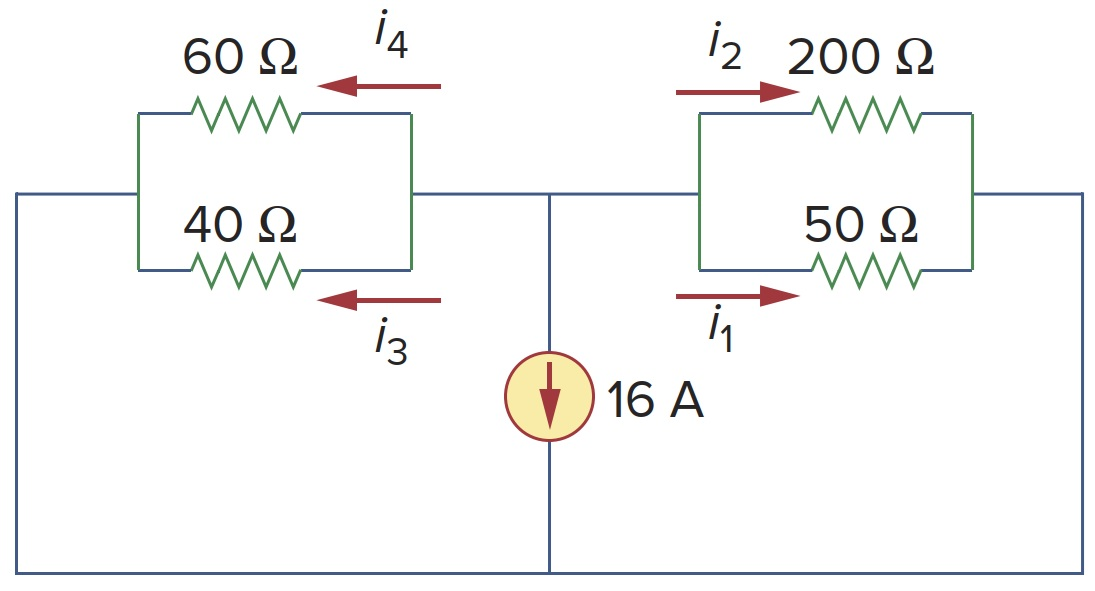
\includegraphics[width=0.46\textwidth]{fig_cir_res2.jpg}
	\caption{Circuit for Problem~\ref{pb:p12}.}
	\label{fig:cir_res2}
\end{figure}
\noindent\makebox[\linewidth]{\color{rouge_poly}{\rule{\textwidth}{1.3pt}}}

\begin{solprob} \text{}\\
    Lets begin by simplifying the circuit by combining the two pairs of resistors to get $R_\text{eq}$.
    \[R_\text{eq1} = \frac{1}{\frac{1}{40} + \frac{1}{60}} = 24\Omega\]
    \[R_\text{eq2} = \frac{1}{\frac{1}{200} + \frac{1}{50}} = 40\Omega\]
    Now, lets solve for the currents going into each equivalent resistor using current division.
    \[I_\text{24$\Omega$} = \frac{40}{24+40}(16\text{A}) = -10 \text{A (taking into account current direction)}\]
    \[I_\text{40$\Omega$} = \frac{24}{24+40}(16\text{A}) = -6 \text{A(taking into account current direction)}\]

    Now, lets solve for each individual current using current division.

    \[i_1 = \frac{200}{250}(-6 \text{A}) = -4.8 \text{A}\]
    \[i_2 = \frac{50}{250}(-6 \text{A}) = -1.2 \text{A}\]
    \[i_3 = \frac{60}{100}(-10 \text{A}) = -6 \text{A}\]
    \[i_4 = \frac{40}{100}(-10 \text{A}) = -4 \text{A}\]

    \[\therefore i_1 = -4.8\text{A}, i_2 = -1.2\text{A}, i_3 = -6\text{A}, i_4 = -4\text{A}\]
    
\end{solprob}

\noindent\makebox[\linewidth]{\color{rouge_poly}{\rule{\textwidth}{1.3pt}}}	
%%%%%%%%%%%%%%%%%%%%%%%%%%%%%%%%%%%%%%%%%%%%%%%%%%%%%%%%%%%%%%%%%%%%%%%%%%%%%%%%%%%%%%%%%%%%%%%%%%%%%%%%%%%%%%
%%%%%%%%%%%%%%%%%%%%%%%%%%%%%%%%%%%%%%%%%%%%%%%%%%%%%%%%%%%%%%%%%%%%%%%%%%%%%%%%%%%%%%%%%%%%%%%%%%%%%%%%%%%%%%
%%%%%%%%%%%%%%%%%%%%%%%%%%%%%%%%%%%%%%%%%%%%%%%%%%%%%%%%%%%%%%%%%%%%%%%%%%%%%%%%%%%%%%%%%%%%%%%%%%%%%%%%%%%%%%
%%%%%%%%%%%%%%%%%%%%%%%%%%%%%%%%%%%%%%%%%%%%%%%%%%%%%%%%%%%%%%%%%%%%%%%%%%%%%%%%%%%%%%%%%%%%%%%%%%%%%%%%%%%%%%	

\begin{prob}\label{pb:p13}
	Find $V_o$ in the circuit in Fig.~\ref{fig:cir_res3} and the power absorbed by the dependent source.
\end{prob}

\begin{figure}[H]
	\centering
	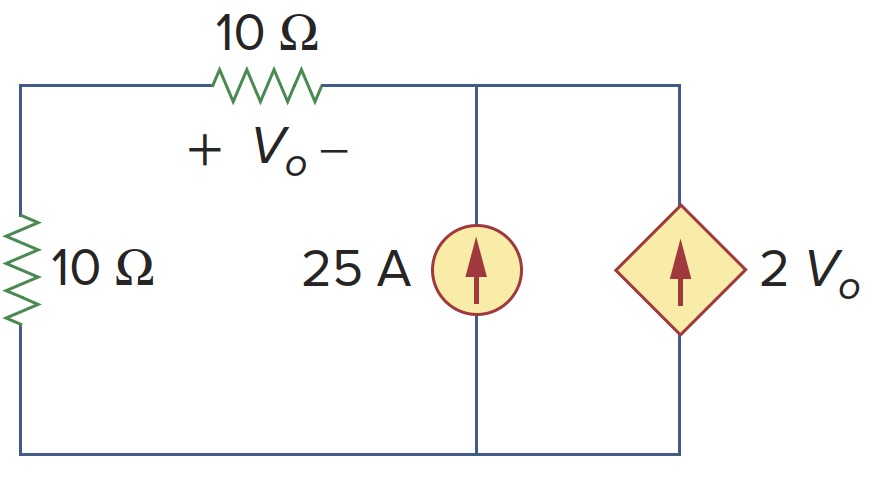
\includegraphics[width=0.46\textwidth]{fig_cir_res3.jpg}
	\caption{Circuit for Problem~\ref{pb:p13}.}
	\label{fig:cir_res3}
\end{figure}

\noindent\makebox[\linewidth]{\color{rouge_poly}{\rule{\textwidth}{1.3pt}}}

\begin{solprob} \text{}\\
    To begin this problem, lets do KCL on the top middle node, then, solve for $I_1$.
    \[25 + 2V_o + I_1 = 0\]
    \[i_1 = -25-2V_o\]
    Now, lets use Ohm's law on the 10$\Omega$ resistor on the top.
    \[V_o = 10I_o = 10(-25-2V_o) = -250-20V_o\]
    \[21V_o = -250\]
    \[V_o = -11.90 \text{ V}\]
    Now that we have $V_o$, we can solve for the dependent current on the right.
    \[i_\text{dep} = 2V_o\]
    \[i_\text{dep} = 2(-11.90) = -23.809\text{ A}\]
    Now, lets calculate the power absorbed by the dependent source. Now, knowing that there is a second resistor, the actual voltage leaving the left wire and entering the two right sources is 2$V_o$, so in the power equation, I will use $v$ as the variable to denote this.
    \[p = -vi = -2(-11.90 \text{ V})(23.809 \text{ A})\]
    \[p = 566.92\text{ W}\]
    \[\therefore \text{the power absorbed by the dependent source is 566.92 W}\]
\end{solprob}

\noindent\makebox[\linewidth]{\color{rouge_poly}{\rule{\textwidth}{1.3pt}}}	
%%%%%%%%%%%%%%%%%%%%%%%%%%%%%%%%%%%%%%%%%%%%%%%%%%%%%%%%%%%%%%%%%%%%%%%%%%%%%%%%%%%%%%%%%%%%%%%%%%%%%%%%%%%%%%
%%%%%%%%%%%%%%%%%%%%%%%%%%%%%%%%%%%%%%%%%%%%%%%%%%%%%%%%%%%%%%%%%%%%%%%%%%%%%%%%%%%%%%%%%%%%%%%%%%%%%%%%%%%%%%
%%%%%%%%%%%%%%%%%%%%%%%%%%%%%%%%%%%%%%%%%%%%%%%%%%%%%%%%%%%%%%%%%%%%%%%%%%%%%%%%%%%%%%%%%%%%%%%%%%%%%%%%%%%%%%
%%%%%%%%%%%%%%%%%%%%%%%%%%%%%%%%%%%%%%%%%%%%%%%%%%%%%%%%%%%%%%%%%%%%%%%%%%%%%%%%%%%%%%%%%%%%%%%%%%%%%%%%%%%%%%	

\begin{prob}\label{pb:p14}
	For the circuit in Fig.~\ref{fig:amp4}, find $V_o / V_s$ in terms of $\alpha$, $R_1$, $R_2$, $R_3$, and $R_4$. If $R_1 = R_2 = R_3 = R_4$, what value of $\alpha$ will produce $|V_o / V_s| = 10$?
\end{prob}

\begin{figure}[H]
	\centering
	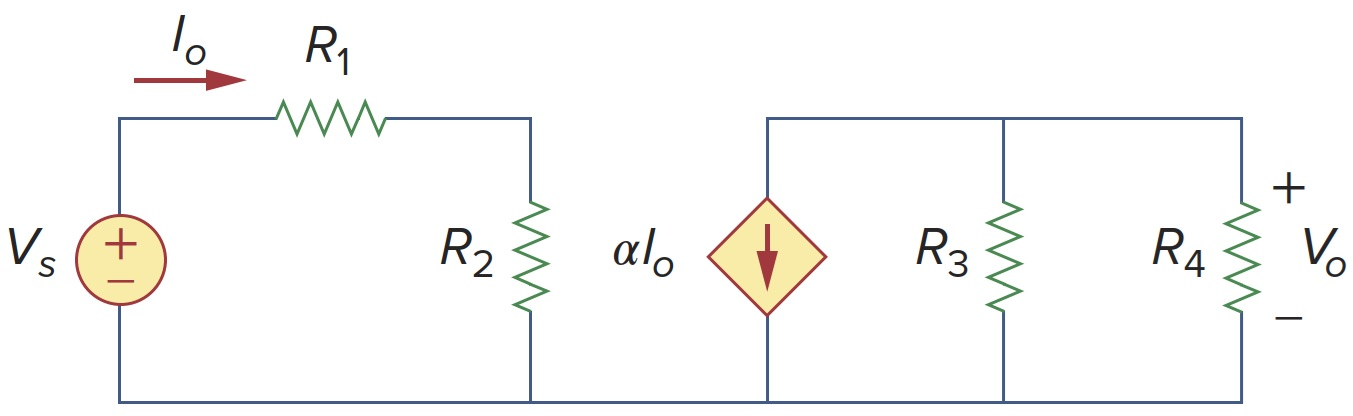
\includegraphics[width=0.6\textwidth]{fig_amp4.jpg}
	\caption{Circuit for Problem~\ref{pb:p14}.}
	\label{fig:amp4}
\end{figure}


\noindent\makebox[\linewidth]{\color{rouge_poly}{\rule{\textwidth}{1.3pt}}}

\begin{solprob} \text{}\\
    Lets begin by using Nodal Analysis.
    \[\frac{V_s-v}{R_1} = I_o\]
    \[I_o = v(\frac{1}{R_2} + \frac{1}{R_3} + \frac{1}{R_4}) + \alpha I_o\]
    \[\frac{V_s-v}{R_1} = v(\frac{1}{R_2} + \frac{1}{R_3} + \frac{1}{R_4}) + \alpha (\frac{V_s-V}{R_1})\]
    \[\frac{V_s-v}{R_1} - \alpha (\frac{V_s-V}{R_1}) = v(\frac{1}{R_2} + \frac{1}{R_3} + \frac{1}{R_4})\]
    \[(1-\alpha)\frac{V_s-v}{R_1} = v(\frac{1}{R_2} + \frac{1}{R_3} + \frac{1}{R_4})\]
    \[(1-\alpha)(V_s-v) = R_1v(\frac{1}{R_2} + \frac{1}{R_3} + \frac{1}{R_4})\]
    \[V_s(1-\alpha)-v(1-\alpha) = R_1v(\frac{1}{R_2} + \frac{1}{R_3} + \frac{1}{R_4})\]
    \[V_s(1-\alpha) = v(1-\alpha) + R_1v(\frac{1}{R_2} + \frac{1}{R_3} + \frac{1}{R_4})\]
    \[V_s(1-\alpha) = v((1-\alpha) + R_1(\frac{1}{R_2} + \frac{1}{R_3} + \frac{1}{R_4}))\]
    \[\frac{v}{V_s} = \frac{(1-\alpha)}{(1-\alpha) + R_1(\frac{1}{R_2} + \frac{1}{R_3} + \frac{1}{R_4})}\]
    \[\frac{v}{V_s} = \frac{1-\alpha}{(1-\alpha) + (\frac{R}{R} + \frac{R}{R} + \frac{R}{R})}\]
    \[\frac{v}{V_s} = \frac{1-\alpha}{1-\alpha + 3} = \frac{1-\alpha}{4-\alpha}\]
    Now that we have this equation, we have to solve for case 1 and 2 for the absolute value function.
    \[|\frac{1-\alpha}{4-\alpha}| = 10\]
    Case 1:
    \[\frac{1-\alpha}{4-\alpha} = 10\]
    \[1-\alpha = 40-10\alpha\]
    \[9\alpha = 39\]
    \[\alpha = \frac{39}{9} = \frac{13}{3}\]
    Case 2:
    \[\frac{1-\alpha}{4-\alpha} = -10\]
    \[1-\alpha = -40 + 10\alpha\]
    \[-11\alpha = -41\]
    \[\alpha = \frac{41}{11}\]
    \[\therefore \text{$\alpha$ needs to be either $\frac{13}{3}$ or $\frac{41}{11}$ for the value of $\frac{V_o}{V_s}$ to be equal to 10.}\]
\end{solprob}

\noindent\makebox[\linewidth]{\color{rouge_poly}{\rule{\textwidth}{1.3pt}}}	
%%%%%%%%%%%%%%%%%%%%%%%%%%%%%%%%%%%%%%%%%%%%%%%%%%%%%%%%%%%%%%%%%%%%%%%%%%%%%%%%%%%%%%%%%%%%%%%%%%%%%%%%%%%%%%
%%%%%%%%%%%%%%%%%%%%%%%%%%%%%%%%%%%%%%%%%%%%%%%%%%%%%%%%%%%%%%%%%%%%%%%%%%%%%%%%%%%%%%%%%%%%%%%%%%%%%%%%%%%%%%
%%%%%%%%%%%%%%%%%%%%%%%%%%%%%%%%%%%%%%%%%%%%%%%%%%%%%%%%%%%%%%%%%%%%%%%%%%%%%%%%%%%%%%%%%%%%%%%%%%%%%%%%%%%%%%
%%%%%%%%%%%%%%%%%%%%%%%%%%%%%%%%%%%%%%%%%%%%%%%%%%%%%%%%%%%%%%%%%%%%%%%%%%%%%%%%%%%%%%%%%%%%%%%%%%%%%%%%%%%%%%	

\begin{prob}\label{pb:p15}
	Find $i$ and $V_o$ in the circuit of Fig.~\ref{fig:cir_res4}.
\end{prob}

\begin{figure}[htbp]
	\centering
	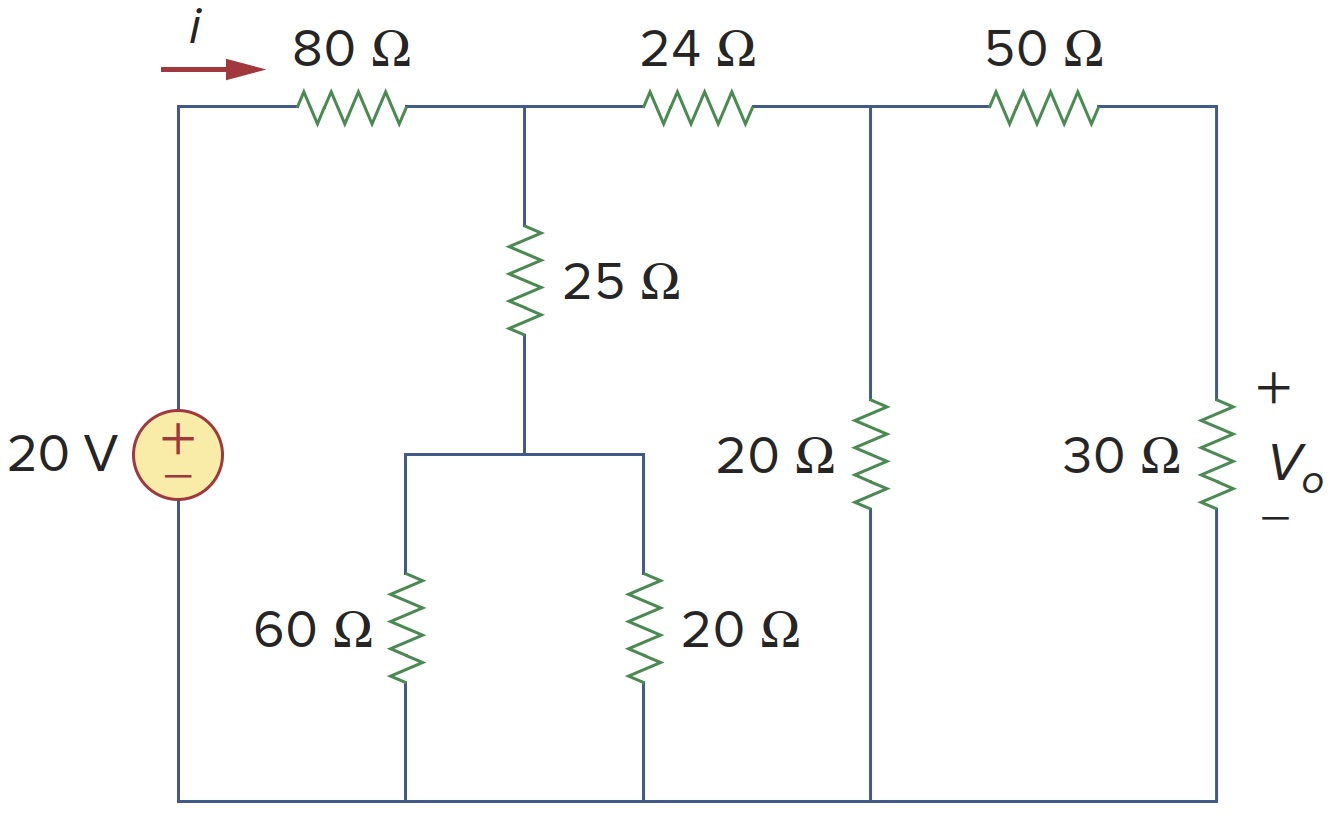
\includegraphics[width=0.6\textwidth]{fig_cir_res4.jpg}
	\caption{Circuit for Problem~\ref{pb:p15}.}
	\label{fig:cir_res4}
\end{figure}

\noindent\makebox[\linewidth]{\color{rouge_poly}{\rule{\textwidth}{1.3pt}}}

\begin{solprob} \text{}\\
    The first step is to simplify the resistors in the circuit to its smallest point. To solve, I'm going to use a few Equivalent resistance equations to calculate the current.
    \[R_\text{$eq_1$} = 50\Omega + 30\Omega = 80\Omega\]
    \[R_\text{$eq_2$} = \frac{1}{\frac{1}{20} + \frac{1}{80}} = 16\Omega\]
    \[R_\text{$eq_3$} = \frac{1}{\frac{1}{20} + \frac{1}{60}}\]
    \[R_\text{$eq_4$} = 25\Omega + 15\Omega = 40\Omega\]
    \[R_\text{$eq_5$} = 24\Omega + 16\Omega = 40\Omega\]
    \[R_\text{$eq_6$} = \frac{1}{\frac{1}{40} + \frac{1}{40}} = 20\Omega\]
    \[R_\text{eq} = 80\Omega + 20\Omega = 100\Omega\]
    Now, with the equivalent resistance, we can solve for i using Ohm's law.
    \[I = \frac{V}{R} = \frac{20\text{ V}}{100\Omega} = 0.2\text{ A}\]
    Now, we need to solve the equation backwards, calculating current division each time until we learn what the $V_o$ current.
    \[I_\text{$24\Omega$} = \frac{40}{40 + 40}(0.2) = 0.1\text{ A}\]
    \[I_\text{$V_o$} = \frac{20}{80+20}(0.1) = 0.02 \text{ A}\]
    Now we solve for $V_o$.
    \[V_o = I_\text{$V_o$}(30\Omega) = (0.02\text{ A})(30\Omega) = 0.6\text{ V}\]\
    \[\therefore \text{$i = 0.2 \text{A and } V_o = 0.6\text{ V}$}\]

\end{solprob}

\noindent\makebox[\linewidth]{\color{rouge_poly}{\rule{\textwidth}{1.3pt}}}	

\end{document}